\documentclass[journal]{IEEEtran}
%\documentclass{article}
%\usepackage[margin=1in]{geometry}
%\usepackage{multicol}


\title{Collaborative Learning with Dirichlet Process Clustering for Rapid Online Adaptation in Robotics}
\author{Runjun Mao \\ August 12, 2023 \\ Supervised by Antoine Cully}
%\date{August 12, 2023}


\usepackage{bm}
%\usepackage{amssymb}
\usepackage{multirow}
\usepackage{booktabs}
\usepackage[T1]{fontenc}
\usepackage{amsmath,amsfonts}
\usepackage{algorithmic}
\usepackage{algorithm}
\renewcommand{\algorithmiccomment}[1]{\hfill $\triangleright$ #1}
\usepackage{array}
\usepackage[caption=false,font=normalsize,labelfont=sf,textfont=sf]{subfig}
\usepackage{textcomp}
\usepackage{stfloats}
\usepackage{url}
\usepackage{verbatim}
\usepackage{graphicx}
\usepackage{cite}
\usepackage{hyperref}
\hypersetup{hidelinks}
%\usepackage[colorlinks, linkcolor=blue, citecolor=green, urlcolor=red]{hyperref}


\begin{document}
\maketitle

\begin{abstract}
\noindent
Robots in deployment can face unforeseeable distortion in their motion due to unseen environment or hardware failures. 
Model-based online adaptation learns this distortion from the interactions with the current environment and corrects its motions accordingly. However, this can be very challenging as it is hard to select the most suitable model and its hyper-parameters for the current dynamics with little prior knowledge.
If we could leverage the plentiful historical real-world interactions, we may build statistical models for the common types of dynamics faced by the robot, hence providing guidance for adaptations. 
This paper developed a method to enable fast online adaptation for the robot by grouping up historical  interaction data into clusters. 
The historical data can be collected from several robots of the same design performing different tasks in different environments, hence allowing learning in a collaborative manner. 
The method takes an non-parametric approach of novelty by modelling the data distribution with infinite mixture of Gaussian Processes and conducting clustering using Dirichlet Processes. 
This achieves unbiased training while ensures high efficiency in terms of both data and computation during deployment. 
The experiment is conducted on a simulated robot to compare with the previous work for online adaptation. 
The method accurately groups up the collaboratively collected data without any knowledge of their sources, and it offers a significant improvement over the baseline in both the efficiency of learning the distortion and the capability of adaptation. 

\end{abstract}


%\begin{multicols}{2}

\section{Introduction}
Locomotion controls of legged robots are typically too complex to be designed manually.
In recent years, deep Reinforcement-Learning (deep RL) has made huge success in game playing
\cite{alphaGo, alphaStar} and is regarded promising for application in robotics. However, training such well performing agents requires enormous amounts of interactions with the environment, meaning that this can only 
be done in simulation where we can model the interaction and collect the training data much faster than in real-time. This raises a problem for application in robotics since there is always a gap between simulation and reality, and the policy trained in simulation could suffer from this sim-to-real transfer. Another problem is that any unforeseen changes to the environment dynamics could lead to severely degraded performance. These deep RL trained agents require extra fine-tuning or even retaining to retain their capabilities.
For example, the team of OpenAI Five \cite{openAI5} had to conduct three additional amendments in the architecture followed by extra trainings to incorporate small version updates in Dota 2 during the development of the agent.
For game-playing agents, these drawbacks are tolerable as there is no sim-to-real problem, and the environment is overall stationary. For robotics however, sim-to-real must be considered, and the environment dynamics is typically non-stationary as the robot can be travelling between different terrain, carrying different payloads or suffering from damages in its hardware.


It would be better if we may learn the true dynamics from the interactions with the current dynamics and
correct our policy accordingly. This is a model-based reinforcement learning (MBRL) solution that allows robots to learn policies with lesser interactions by learning a dynamics model and use it optimize the policy \cite{MBRL, black_box_search, policy_search}. 
However, the amount of data required to learn a model typically scales exponentially with the dimensionality of the input space \cite{curse_of_dim}, hence it is not suitable for online adaptation. 
The promising approach to address this is to use a repertoire-based method, where we learn a repertoire of elementary policies (e.g., one policy for turning left, one for moving forward, etc.) using quality diversity optimisation \cite{QD} to fully cover the task space (e.g., the 2D displacement we want the robot to make). 
The repertoire-based method is a hierarchical control method that keeps a variety of elementary policies and treats each policy as an action. 
We then give each elementary policy a behaviour descriptor (BD) to quantify the way it acts.
This enables us to skip the low-level states and actions (i.e., joint encoders and torques for all motors) and to work with the high-level behaviour space that has much smaller dimensionality.
During the adaptation, we learn the distortion (called transformation model) in the behaviour space from real-world interactions. Thanks to the reduced dimensionality, the transformation model can be learned in real-time.
Instead of optimising the policy with this learned model, we use a repertoire-based control that first predicts the outcomes for each elementary policy in the repertoire and then simply chooses the one with the predicted outcome that is most aligned with the current goal. 
This is made available for keeping a repertoire of policies rather than a single policy, so that the robot can adapt to the distortion by finding the corresponding policies that compensate the distortion (for example the robot aims to go forward and distortion is left, then a policy originally aiming right-front can be used for going forward instead).


The repertoire-based method has achieved very impressing results in task-solving \cite{EvoRBC} and online damage recovery \cite{RTE}. 
But this method heavily relies on having a good model that is both data efficient and suitable for modelling the distortion. 
The most commonly used model is Gaussian Process (GP) \cite{GP}. The prior mean function and the kernel are the most important factors of GP. 
If no prior knowledge is given about the dynamics, these  have to be selected manually according to experience.
If the distortion is very large (like broken legs) or complex, the GPs can be very inefficient or even misleading.
If we have data of real-world interactions across several different environments, we can build a GP for each of the situations and then teach the robot to identify the one that mostly explains its current situation. However, such real-world data are expensive to collect and could lead to covariate shift (the collected data distribution is different from that during deployment).
A promising solution that is to leverage the historical data of real-world interactions collected during deployment. 
After performing each task, the interaction data can be uploaded to an archive system where they will be analysed. 
Thus, the data doesn't have to be collected on purpose, and the acquired data distribution is completely unbiased. 
This also allows the robots to learn to adapt in a collaborative manner.
If we have multiple robots performing different tasks in different environments, we can quickly get an overview of the  common types of dynamics and build the adaptation strategy accordingly. 
If a robot encounters a new environment, with the interaction data uploaded, all the robots will be able to quickly adapt to this environment.
Finally, considering the scalability of such system, we can group the data into clusters based on their dynamics and assign a GP (with the corresponding mean and kernel) to each cluster. This prevents the adaptation strategy from becoming computationally expensive after we have collected data from thousands of tasks.

There are many challenges needs to be addressed to enable this collaborative learning. First, traditional clustering algorithms like k-nearest neighbours \cite{knn} and k-means \cite{k-means} need to specify the number of clusters. While in our case, this number is not even fixed as we might observe more clusters as we collect more data.
Second, we know that each task corresponds to a single environment, and hence we are essentially clustering the tasks instead of clustering the data points.
However, since some tasks are tougher than others, different tasks generate different amount of data. 
As a result, we will be clustering data of inconsistent sizes.
Third, since there is a large repertoire of policies, only a small subset of them will be executed while performing each task. Hence, it is very likely that the data collected from two tasks have no overlapping policies, making it hard to determine whether they have similar dynamics and whether they should be grouped together.
Moreover, after we have found the clusters, the data in each cluster can never cover the entire repertoire. Hence it is difficult to determine the prior mean for the policies that are not present in this cluster.
This paper aims to solve all the above problems by taking an non-parametric clustering method and using a uniquely designed prior mean function.


\section{Related Works}
\subsection{Quality-Diversity Optimization}
The repertoire-based method uses quality diversity (QD) optimization to generate a repertoire of diversified and high-quality locomotion behaviours. 
The most popular method for doing QD is called MAP-Elites \cite{QD, Map-Elites}, where we tabularize the task-space (for example, discretize the displacement of the robot along the x, y axis) into grids. 
Each grid corresponds to a policy that leads the robot to this part of task space. 
Initially the grids are empty, as we have no policies at start, and will be filled during a process of stochastic optimization inspired by natural evolutionary. 
We start from a few random policies, which are typically neural networks, and execute them in the simulator to get their outcomes in the task space. 
We also assign a performance score (called fitness) to each policy to quantify the efficiency of the execution. Typically, the fitness can be based on the energy consumption \cite{Q-Dax} or the shape of the trajectory \cite{evorbc_conf}.
Each of these outcomes is mapped to one of the girds (hence these grids are filled). 
We then begin our main loop of policy generation. 
In each iteration we select a few policies corresponding to the filled grids as the parents. We then conduct crossover on the parents to mutate their genotypes (for neural networks, these are just the weights of the neurons) to get their off-springs. 
The crossover operation should balance the exploitation and exploration by ensuring some inheritance of the parents to preserve good genes as well as some random variations for promoting diversity.
We then evaluate the off-springs in the simulator to get their outcomes in the task space and identify the grids they belong to.
If a grid is already occupied by another policy, we only keep the one with the higher fitness; if it is empty, we fill this grid with the corresponding off-spring. 
The pseudo code for MAP-Elites QD algorithm is presented below.

\begin{algorithm}
\caption{MAP-Elites}
\begin{algorithmic}
\STATE \textbf{procedure} MAP-Elites
\STATE Discretize the task space into grids
\STATE $\mathcal{R} \leftarrow \emptyset$ \COMMENT{Initialize repertoire}
\FOR{$\bm{i} = 1 \rightarrow G$}
\STATE $\theta \leftarrow $ generate{\_}random{\_}policy()
\STATE $\Theta$, $f$ $\leftarrow$ evaluate{\_}policy($\theta$) \COMMENT{Get outcome and fitness}
\STATE add{\_}to{\_}repertoire($\Theta$, $f$, $\theta$, $\mathcal{R}$) \COMMENT{Update repertoire}
\ENDFOR
\FOR{$\bm{i} = 1 \rightarrow T$}
\STATE $\vartheta \leftarrow$ select{\_}parents($\mathcal{R}$)
\STATE $\bm{\theta} \leftarrow$ crossover($\vartheta$, $N$) \COMMENT{Generate $N$ off-springs}
\FOR{$\bm{j} = 1 \rightarrow N$}
\STATE $\Theta$, $f$ $\leftarrow$ evaluate{\_}policy($\bm{\theta_j}$)
\COMMENT{Off-spring evaluation}
\STATE add{\_}to{\_}repertoire($\Theta$, $f$, $\bm{\theta_j}$, $\mathcal{R}$)
\ENDFOR
\ENDFOR
\end{algorithmic}
\label{MAP-Elites}
\end{algorithm}
\noindent
Evaluating the policies in the simulation is the major source of computationally expense for the MAP-Elites.
A merit of this algorithm is that the inner for loop of off-spring evaluation can be conducted in parallel, and the repertoire update can be made after having collected all the results of the off-springs.
This enables us to generate a large number of off-springs in each iteration and evaluate them in parallel, fully leveraging the power of modern Cluster computing \cite{Q-Dax}.
By running the algorithm for a few thousand iterations, we will end up having a repertoire of high-performing policies well-covering the task space.

\subsection{Gaussian Process}
The Gaussian Process (GP) is a powerful non-parametric machine learning algorithm. 
It assumes the prior distribution of the outcomes to be a multivariate normal distribution with a prior mean $\mu$ and a covariance matrix $\Sigma$. 
\begin{equation}
f(\bm{y}) = \frac{exp(
-\frac{1}{2}(\bm{y} - \bm{\mu})^T \bm{\Sigma^{-1}} (\bm{y} - \bm{\mu})
)}
{
\sqrt{(2\pi)^N \det(\bm{\Sigma})}
}
\label{multi_normal}
\end{equation}
In contrast to regular multivariate normal distribution, GP allows the prior mean and the covariance matrix to be input dependent. The
prior mean becomes a function $\mu(\bm{x})$, and the covariance between two data points is given by a covariance function 
$k(\bm{x_1}, \bm{x_2})$ called kernel. 
Following the fact that data points closer to each other are more correlated, this covariance starts from the prior variance and asymptotically decreases to zero as the distance between the two points tends to infinity. 
To account for the fact the observations might be noisy, we can incorporate the noise into the covariance matrix by adding the variance of the noise on the diagonal.
\begin{equation}
\bm{\Sigma} = \bm{K}(\bm{x_{1:N}}, \bm{x_{1:N}}) + \sigma_n^2 \mathbf{I}
\label{covariance_matrix}
\end{equation}

This allows us to build reasonable joint prior distribution for the values of any well-behaved functions.
To make prediction with GP, we first use the prior mean function and kernel to build up the joint distribution as the prior. 
Then we can calculate the posterior for the data we wish to evaluate conditioned on the ones we have observed using Bayes rule.
Since the Gaussian distribution is a conjugate distribution, the posterior is still a Gaussian with mean and variance given by \cite{GP, GP_posterior}:
\begin{equation}
\begin{gathered}
\mu_*(x) = \mu(x) + 
\bm{\Sigma}_{N, x}^T
\bm{\Sigma}_{N, N}^{-1}
(\bm{y}_{1:N} - \bm{\mu}(\bm{x}_{1:N}))
\\
\sigma^2_*(x) = \sigma^2(x) -  
\bm{\Sigma}_{N, x}^T
\bm{\Sigma}_{N, N}^{-1}
\bm{\Sigma}_{N, x}
\end{gathered}
\label{GP_posterior}
\end{equation}
where $\bm{\Sigma}_{N, N}$ denotes the covariance matrix of the observed data, and $\bm{\Sigma}_{N, x}$ denotes the column vector with entry on each row equal to the covariance between 
each observed data and the data we hope to evaluate.

Typically, the prior mean is just a fixed constant like zero, representing the prior knowledge we have about the outcome when there is no neighbouring data to refer to.
The typical choice of kernel can be RBF kernel that models the correlations to decrease in the form of a Gaussian function.
\begin{equation}
k(\bm{x_i}, \bm{x_j}) = \alpha_0 e^{-\frac{1}{2} d_{ij}^2}
\label{RBF_kernel}
\end{equation}
RBF kernel assumes the function is infinitely differentiable, which may be factually incorrect. Hence, it might be more desirable to use the Matern kernel:
\begin{equation}
k(\bm{x_i}, \bm{x_j}) = \alpha_0 \frac{2^{1-v}}{\Gamma(v)}
(\sqrt{2v} d_{ij})^v K_v(\sqrt{2v} d_{ij})
\label{Matern}
\end{equation}
where the $\Gamma$ is the gamma function, and the $K_v$ is the modified Bessel function of the second kind. The $v$ controls the smoothness, as GP using Matern kernel is $\lceil v \rceil - 1$ times differentiable in the mean-square sense \cite{GP, Matern}.
The distance $d_{ij}$ between two data points does not have to be Euclidean distance. A more general form would be:
\begin{equation}
d_{ij}^2 = \Sigma_{d=1}^D \frac{(x_{d, i} - x_{d, j})^2}{l_d^2}
\label{distance_metric}
\end{equation}
Where this distance metric can be anisotropic, suggesting distance along some axis contributes more uncertainty than others. 
The $l_d$ in the denominator is a positive number called length scale that determines how slowly we lose uncertainty (bigger length scale means the function is flatter) along the $d^\text{th}$ axis.

\subsection{Reset-free Trial-and-Error Learning}
The work of this paper is based on the Reset-free Trial-and-Error \cite{RTE} (RTE) algorithm. 
The RTE uses GP to learn the transformation model online.
This is a very clever choice for two reasons.
First, the online learning requires very high data-efficiency, which happens to be one of the strengths of GP. 
Secondly, the true dynamics happens at low level, while the repertoire-based method learns the transformation model at high level. This will inevitably introduce errors, which can be well incorporated by GP as being a probabilistic model.
In RTE, the task space is just the displacement of the robot in x and y direction after executing each policy.
The prior mean function of RTE is chosen to be the outcomes of the policies evaluated in the simulator, which are the results collected during the MAP-Elites policy generation. 
Since the policy outcome has two dimensions (x and y), RTE uses a different GP for each dimension.
The kernel is chosen to be the RBF kernel with an isotropic distance metric. The input space is chosen to be the same as the task space, namely the x and y displacement evaluated in the simulation. 
During online adaptation, the RTE first predicts the outcome of each policy in the repertoire using Eq. (\ref{GP_posterior}), then it uses a Monte Carlo Tree Search \cite{MCTS} (MCTS) to plan its actions.
It is worth noting that the RTE uses a periodic set of commands as the elementary policy. 
This means the policy execution is open-loop control, despite the robot knows its position and orientation.
While using such periodic controllers seems to be weaker than using a neural network, it is much more stable than using neural networks. 
This is because a periodic controller performs all its actions during evaluation, while neural networks are much more complicated and could behave very differently in different situations.
Since the repertoire based control aims to learn the distortion with limited number of interactions, the distortion cannot be too large or too complicated. Hence the use of periodic controller is a much better choice. 


This method is not very ideal for three reasons. 
First, the use of outcomes in default simulation setting as the prior mean is not good enough. Since some conditions like broken leg can lead to very large distortions. In this case, such prior would be misleading. 
Second, the use of the task space as the input space is not ideal. Two policies leading to very close displacements could follow very different trajectories, hence they may react very differently to the same new environment.
Also, the kernel in the RTE is manually chosen, which depends on experiences of the designer and could lead to suboptimal results.
Nevertheless, this method successfully enabled a damaged hexapod robot to recover 77.52\% of its capability \cite{RTE} and significantly outperforms the baseline result that does not use the GP as the transformation model.
Some other works like Adaptive Prior selection for Repertoire-based Online Learning \cite{APROL} (APROL) take very similar approach as RTE but use several repertoires generated in different environments to address potential large distortions. 
Since RTE is easier to implement, and any improvements on the RTE can be easily transferred to other other works, it is selected as the algorithm that our work is based on.

\subsection{Dirichlet Process Mixture Model}
Dirichlet process mixture model (DPMM), also called infinite mixture model, is a Bayesian non-parametric model widely used in data clustering. 
It is based on a stochastic process called Dirichlet Process (DP).
DP assumes that the data are sampled from a distribution of distributions. For example, the data points come from a set of Gaussian distributions, while the mean and variance of each Gaussian follow another distribution. 
To make clear explanation, we first investigate the finite mixture model using DP, and then extend the derivations to the infinite limit.
We know that finite mixture models can be represented as:
\begin{equation}
p(\bm{y}) = \Sigma_{j=1}^k \pi_j \cdot p(\bm{y}|\bm{\theta_j})
\label{finite_mixture_model}
\end{equation}
where this model consists of $k$ components, and $\bm{\theta_j}$ and $\pi_j$ are the parameters and the mixture weights (also called mixing proportions) for each mixture component.
DP assumes the parameters and the mixture weights are independently sampled. 
The parameters of the mixture components are sampled from a base distribution $H$, and the mixture weights are sampled from a symmetric Dirichlet distribution \cite{DP}:
 \begin{equation}
p(\pi_1, \dots, \pi_k | \alpha) = 
\frac{\Gamma(\alpha)}{\Gamma(\alpha / k)^k} \prod_{j=1}^k \pi_j^{a/k - 1}
\label{Dirichlet_distribution}
\end{equation}
Where the mixture weights are positive and sum up to 1. The constant $\alpha$ is called concentration parameter, which controls how dense the sampling will be.
To train a DPMM, the only thing we need to determine is the indicator of each data which points to the mixture component that this data belongs to. 
We then try to find the configuration of the indicators that maximizes the posterior likelihood (MAP estimate). 
This is very hard to do directly, typical alternative approaches include Gibbs sampling \cite{Gibbs_sampling, Gibbs} and the use of variational inference \cite{variational_method}.
This paper uses the Gibbs sampling method. 
In each iteration, we loop through each indicator and resample it based on the other indicators:
\begin{equation}
\begin{gathered}
p(c_i = j|y_i, \bm{y}_{-i}, \bm{c}_{-i}, \alpha) 
\propto  \\
p(c_i = j|\bm{c}_{-i}, \alpha) \cdot
p(y_i|c_i=j, \bm{y}_{-i}, \bm{c}_{-i})
\end{gathered}
\label{indicator_posterior}
\end{equation}
%
The subscript $-i$ means all the data except for $i$.
We know the probability of getting a certain configuration is:
\begin{equation}
p(c_1,\dots, c_n|\pi_1, \dots, \pi_k) = \prod_{j=1}^k \pi_j^{n_j}
\label{configuration_probability}
\end{equation}
Where the $n_j$ in the superscript denotes the number of data assigned to the $j^\text{th}$ component.
Using Eq. (\ref{Dirichlet_distribution}) and standard Dirichlet integral, we can calculate the probability density of such configuration in the prior:
\begin{equation}
\begin{gathered}
p(c_1, \dots, c_n | \alpha) =  \frac{\Gamma(\alpha)}
{\Gamma(\alpha / k)^k} \int \prod_{j=1}^k \pi_j^{n_j + a/k - 1} d\bm{\pi}
\\
= \frac{\Gamma(\alpha)}{\Gamma(\alpha + n)} 
\prod_{j=1}^k \frac{\Gamma(n_j + \alpha/k)}{\Gamma(\alpha/k)}
\end{gathered}
\label{indicator_prior}
\end{equation}
Hence we can find the posterior using Bayes rule:
\begin{equation}
p(c_i =j | \bm{c}_{-i} , \alpha) = 
\frac{n_{-i, j} + \alpha /k}{\alpha + n - 1}
\label{indicator_posterior_2}
\end{equation}
%
So far, we have been discussing the case of finite mixture models. If we let the component number $k$ tend to infinity, we will have the equations for infinite mixture models:
\begin{equation}
\begin{gathered}
p(c_i =j | \bm{c}_{-i} , \alpha) = 
\frac{n_{-i, j}}{\alpha + n - 1}
\\
p(c_i \neq j \, \text{for any} \, n_j \neq 0 | \bm{c}_{-i} , \alpha) = 
\frac{\alpha}{\alpha + n - 1}
\end{gathered}
\label{indicator_posterior_3}
\end{equation}
For any existing cluster (mixture component with at least one data assigned to it), this probability is proportional to the number of data in that cluster. 
Note that there is a non-zero probability that this data belongs to a new cluster. 
This is a very important property of DPMM that new clusters can be automatically generated based on the likelihood. 
To calculate the last term in Eq. (\ref{indicator_posterior}), we integrate the likelihood over the posterior:
\begin{equation}
\begin{gathered}
p(y_i|c_i, \bm{y}_{-i}, \bm{c}_{-i}) = 
\int p(y_i|\bm{\theta})
p(\bm{\theta}|c_i, \bm{y}_{-i}, \bm{c}_{-i})
d\bm{\theta}
%
\\
%
\text{where \,\,} 
p(\bm{\theta}|c_i, \bm{y}_{-i}, \bm{c}_{-i}) \propto
\,\, p(\bm{\theta})
\prod_{c_k=c_i, k \neq i} p(y_k|\bm{\theta})
\end{gathered}
\label{integral_1}
\end{equation}
In the case of a new cluster, the integration is made over the prior:
\begin{equation}
p(y_i|c_i \neq j \, \text{for any} \, n_j \neq 0) = 
\int p(y_i|\bm{\theta})
p(\bm{\theta})d\bm{\theta}
\label{integral_2}
\end{equation}
To conduct Gibbs sampling, we first start from an initial configuration of indicators (common choice is that every data is a cluster on its own).
Then in each iteration, we loop through each indicator and use Eq. (\ref{indicator_posterior}) to resample it. 
The $-i$ subscript on $\bm{y}$ means we need to remove the data from its current cluster during resampling, which will affect the result of Eq. (\ref{integral_1}) when calculating the probability of the data remaining in its current cluster. 
The Gibbs sampling is a Markov Chain Monte Carlo (MCMC) that satisfies irreducibility, positive recurrence and aperiodicity, hence it will eventually converge to the equilibrium distribution regardless of its initial state \cite{MCMC}. 
Since we are aiming to maximize the posterior likelihood, we need to calculate the likelihood after each iteration and record the configuration with the highest value.
The posterior likelihood is given by:
\begin{equation}
\begin{gathered}
p(\bm{c}|\bm{y}) \propto 
\left[\prod_{n_j \neq 0} \alpha \Gamma(n_j)\right]
\prod_{i=1}^n p(y_i|c_i, \bm{y}, \bm{c}_{-i})
\end{gathered}
\label{posterior_likelihood}
\end{equation}
Note that the probability in the second product doesn't have the $-i$ subscript on $\bm{y}$ like in Eq. (\ref{integral_1}), so the data doesn't need to be removed from its current cluster now.


We also need to define the base distribution $H$ that gives the prior distribution $p(\bm{\theta})$ and the concentration parameter $\alpha$ which controls the generation of new clusters.
Note that under the assumptions of DP, the final data distribution is a biased sample from $H$ unless $\alpha$ tends to infinity. Hence we don't need to ensure our $H$ being close to data distribution, while a rather conservative distribution is encouraged.
The $\alpha$ is selected based on Eq. (\ref{indicator_posterior_3}).
We can see that the probability of getting a new cluster is proportional to $\alpha$ and decreases asymptotically to zero as the number of data increases.
This is reasonable as the more data we have, the more certain we are that we have sampled at least one data from each cluster, hence the lesser we need a new cluster. 
If the $\alpha$ is infinite, DP believes all mixture component has the equal weight, and the data should always belong to a new situation regardless how many data we have collected.
In practice, we can estimate the amount of data we need in order to fully cover all situations. Then we can find the corresponding $\alpha$ using Eq. (\ref{indicator_posterior_3}) so that the probability decreases to a small value (e.g. 1\%) after we have collected this number of data.

DPMM is a very powerful tool to make non-parametric clustering without specifying the number of clusters. 
It can also easily incorporate the infinite limit than approaches working with finite models of unknown sizes like \cite{Bayesian_mixture}.
Comparing with optimization based methods like EM \cite{EM}, the use of MCMC can easily overcome the local optimal \cite{infinite_GMM}. 
For example, if there are duplicated mixture components, EM will still converge but the DPMM will eventually merge them as the Eq. (\ref{posterior_likelihood}) favours the data to be concentrated. 
Note that the above derivations of DPMM did not put any constrain on the type of distribution, namely the term $p(y|\bm{\theta})$ in Eq. (\ref{integral_1}). Such distribution can also be non-parametric distributions like Gaussian Processes. 
This means we can use DP to cluster the dynamics in RTE, which is GP, to build a mixture model of the real-world dynamics.



\section{Methodology}
We are aiming to improve RTE by leveraging the collaboratively collected real-world interactions as the priors of our GP.
The greatest difficulty lies in the way to build the priors.
In GPCF, data from each previous user is treated as one of the candidate priors.
If we are to use the same design, we can use the posteriors calculated (with GP) using the data collected from each single task as the priors.
However, this would not be a very ideal design in our case.
The first reason is that we will be having a large number of priors after we have collected many data.
Second, it is likely that some data many come from similar dynamics and should be grouped together to enable more sophisticated analysis.
Hence, we took a different approach by first clustering the data based on their dynamics and then building a prior for each cluster.
Since the dynamics for each previous deployment is modelled by GP, we can use DP to group them in a non-parametric manner.
The result of such DP clustering will be an infinite mixture of GPs, where each cluster will be a GP with the prior and parameters following a certain posterior distribution.
We then replace the transformation model in RTE by this infinite mixture of GPs, and let the robot identify the most likely GP during real-world adaptation.



Previous works of training infinite mixture of GP using DP clustering have been made in \cite{infinite_MGP, variational_MGP}. 
But in our case, the design needs to be different.
First, our real-world interaction data are produced in individual episodes, where each episode corresponds to the interactions collected during each deployment.
Since we know that each deployment is made in a certain environment, all the interactions in an episode should correspond to the same dynamics. 
Hence, when clustering the historical data we need to conduct clustering on the episode but not on the individual data. 
The second difference from previous works is that we are decoupling each dimension and each episode.
The decoupling of dimension is inherited from RTE, while the decoupling of episodes is a unique design.
This is based on the fact that data within each episode come from the same environment and are hence correlated, while different episodes do not necessarily correspond to the same environment even they are grouped into the same cluster.
Such design allows us to group up environments that are different but similar, providing higher flexibility.
Another reason for using decoupled episodes is to make our system scalable.
Since we are now clustering episodes which typically contains dozens of data, each clusters can have thousands of data.
GP requires to compute the inverse of the joint covariance matrix, which has time complexity scaling cubic with data size.
Such computational expense is completely unaffordable for online adaptation. 
If the episodes are decoupled, the joint covariance matrix becomes a block diagonal matrix, and the time complexity of its inverse scales only linearly.



It can be very hard to design a good prior function or to determine the kernel if we have completely no idea about the real-world dynamics.
Hence, a few parts of our methodology relies on the use of simulation.
For this, the simulation has to be relatively accurate and free of bugs.
We also make a very strong assumption that the simulated results always correspond to real-world outcomes in some environment. 
For example, we set the friction coefficient to 0.9 in the simulation, but the friction is underestimated and the simulated outcomes are very close to the real-world results for friction coefficient equal to 0.8.
Hence we believe that although the simulated results are not strictly accurate, they can still represent some real-world results.
This assumption not always true, but it plays a very important role in the methodology.



\subsection{Linear Prior Mean Function}
In GP, the prior mean function is most important as it provides the prior estimate of the outcomes of all the elementary policies.
To determine a suitable form of the prior mean function, we hope to study the dependencies of the dynamics.
We know that the outcome of a policy should depend on the behaviour of this policy as well as the environment.
Hence, we express the dynamics in the following form:
\begin{equation}
x_d(\bm{\beta}, \bm{\epsilon}) = f_d(\bm{\beta}, \bm{\epsilon}) 
+ g_d(\bm{\beta}) 
+ h_d(\bm{\epsilon}) + c_d 
\label{dynamics_assumption}
\end{equation}
where the $x_d$ stands for the $d^{\text{th}}$ dimension of the policy outcome (for example, this can be the robot displacement in the $x$ axis). Vector $\bm{\beta}$ represents the behaviour descriptor of the controller; vector $\bm{\epsilon}$ is the environment descriptor, representing some quantities of the environment. 
It can be seen from Eq. (\ref{dynamics_assumption}) that the dynamics consists of a term that depends on both the policy behaviour and the environment plus the terms that only depends on either the behaviour or environment plus a constant $c_d$.
Note that we do not require access to the $\bm{\beta}$ and $\bm{\epsilon}$ or knowing their detailed meanings.
Eq. (\ref{dynamics_assumption}) is generally non-linear. But in the case where the dynamics is relatively simple, like the use of periodic controller in RTE, we can get an approximation of it by Taylor expanding the $f_d(\bm{\beta}, \bm{\epsilon})$ term to the second order:
\begin{equation}
\begin{gathered}
f_d(\bm{\beta}, \bm{\epsilon}) \approx
f_d(\bm{\beta}_0, \bm{\epsilon}_0) + 
\begin{bmatrix}
J_{\bm{0, \beta}} & J_{\bm{0, \epsilon}} \\
\end{bmatrix}
%
\begin{bmatrix}
\Delta \bm{\beta} \\
\Delta \bm{\epsilon}
\end{bmatrix}
%
\\
%
+ \frac{1}{2}
\begin{bmatrix}
\Delta \bm{\beta}^T & \Delta \bm{\epsilon}^T \\
\end{bmatrix}
%
\begin{bmatrix}
H_{\bm{0, \beta \beta}} & H_{\bm{0}, \bm{\beta \epsilon}} \\
H_{\bm{0, \epsilon \beta}} & H_{\bm{0, \epsilon \epsilon}} \\
\end{bmatrix}
%
\begin{bmatrix}
\Delta \bm{\beta} \\
\Delta \bm{\epsilon}
\end{bmatrix}
\end{gathered}
\label{Taylor_expansion}
\end{equation}
where the Jacobian vector $J_{\bm{0}}$ and the Hessian matrix $H_{\bm{0}}$ have been arranged in the partitioned form, and their subscript 0 denotes they are evaluated at $(\bm{\beta}_0, \bm{\epsilon}_0)$.
We then substitute this result into Eq. (\ref{dynamics_assumption}) to arrive at:
\begin{equation}
\begin{gathered}
x_d(\bm{\beta}, \bm{\epsilon}) \approx
\Delta \bm{\beta}^T H_{\bm{0, \beta \epsilon}} \Delta \bm{\epsilon}
+ f_d(\bm{\beta}_0, \bm{\epsilon}_0) + c_d
\\ + 
\frac{1}{2} \Delta \bm{\beta}^T H_{\bm{0, \beta \beta}} \Delta \bm{\beta} 
+ J_{\bm{0, \beta}} \Delta \bm{\beta}
+ g_d(\bm{\beta}) 
\\
+ \frac{1}{2} \Delta \bm{\epsilon}^T H_{\bm{0, \epsilon \epsilon}} \Delta \bm{\epsilon}
+ J_{\bm{0, \epsilon}} \Delta \bm{\epsilon}
+ h_d(\bm{\epsilon}) 
\end{gathered}
\label{approximation}
\end{equation}
%
Comparing Eq. (\ref{approximation}) with Eq. (\ref{dynamics_assumption}), we can see our approximation factorizes the correlated term. If the same policy is executed in two different environment, the difference in the dynamics will be:
\begin{equation}
\begin{gathered}
x_d(\bm{\beta}, \bm{\epsilon}_1) - 
x_d(\bm{\beta}, \bm{\epsilon}_2) \approx
\Delta \bm{\beta}^T H_{\bm{0, \beta \epsilon}} 
(\bm{\epsilon}_1 - \bm{\epsilon}_2)
\\
+ h^*_d(\bm{\epsilon}_1) - h^*_d(\bm{\epsilon}_2) 
\\
\text{where \,}
h^*_d(\bm{\epsilon}) = 
\frac{1}{2} \Delta \bm{\epsilon}^T H_{\bm{0, \epsilon \epsilon}} \Delta \bm{\epsilon}
+ J_{\bm{0, \epsilon}} \Delta \bm{\epsilon}
+ h_d(\bm{\epsilon}) 
\end{gathered}
\label{dynamics_diff}
\end{equation}
If we treat the $h^*_d(\bm{\epsilon})$ term as an additional dimension of the environment vector, then Eq. (\ref{dynamics_diff}) can be represented as:
\begin{equation}
\begin{gathered}
\Delta \bm{x}_d = 
\begin{bmatrix}
\Delta x_{d, 1} \\
\vdots \\
\Delta x_{d, N} \\
\end{bmatrix}
\approx
\begin{bmatrix}
\Delta \bm{\beta}_1^T H_{\bm{0, \beta \epsilon}} & 1 \\
\vdots & \vdots \\
\Delta \bm{\beta}_N^T H_{\bm{0, \beta \epsilon}} & 1 \\
\end{bmatrix}
\Delta \bm{\varepsilon} 
\\
= W_{d}^T \Delta \bm{\varepsilon}
\end{gathered}
\label{linear_form}
\end{equation}
where $\bm{\varepsilon}$ is our new environment vector. 
The vector $\Delta \bm{x}_d$ stands for the difference in dynamics for the entire repertoire with each entry $\Delta x_{d, i}$ denoting the result for the each elementary policy.
Combined with the assumption we made about the simulation, Eq. (\ref{linear_form}) suggests we may approximate the real-world distortion of the entire repertoire using a linear model, which is consistent with the design in GPCF.


The above derivations can be extended to any order of Taylor expansion, but the dimension of the new environment vector $\bm{\varepsilon}$ increases exponentially after the second order.
If we assume the dynamics can be efficiently approximated with the second order expansion, Eq. (\ref{linear_form}) gives a very potent result.
However, we do not have access to the matrix $W_d$ or the environment vector $\bm{\varepsilon}$ directly. 
Instead, we can leverage the fact that any environment vector can be linearly represented by a set of environment vectors as the basis.
Hence, if we have collected enough distortions, any new distortion can be  represented with a linear combination of the collected ones:
\begin{equation}
\begin{gathered}
\Delta \bm{x}_d^* \approx
W_{d}^T \Delta \bm{\varepsilon}^* = 
W_{d}^T
\begin{bmatrix}
\Delta \bm{\varepsilon}^{(1)}, \cdots, \Delta \bm{\varepsilon}^{(n)}
\end{bmatrix}
\begin{bmatrix}
\omega_1^* \\
\vdots \\
\omega_n^* \\
\end{bmatrix}
\\ =
\begin{bmatrix}
\Delta \bm{x}_d^{(1)}, \cdots, \Delta \bm{x}_d^{(n)}
\end{bmatrix}
\begin{bmatrix}
\omega_1^* \\
\vdots \\
\omega_n^* \\
\end{bmatrix}
\end{gathered}
\label{linear_combination}
\end{equation}
This means we need to get the distortions of all the elementary policies in several environments.
Since typically a repertoire can contain of a few thousand policies,
we cannot afford to do such amount of evaluations in the real-world, and hence we need to rely on simulation.


A question is that how many distortions we should collect.
If we get too few distortions, we might not have collected all the basis, and the linear model will perform poorly in uncovered environments.
On the other hand, if we have collected too many, not only will this be computationally expensive but this will also lead to very large dimensions. 
The solution is collect as many as we can afford and then reduce the dimensionality with singular vector decomposition (SVD). The collection of distortions can be represented as:
\begin{equation}
\bm{A} = 
\begin{bmatrix}
\Delta \bm{x}_d^{(1)}, \cdots, \Delta \bm{x}_d^{(n)}
\end{bmatrix}
= \sum_{i=1}^s \sigma_i \bm{v}_i \bm{u}_i^T
\label{SVD}
\end{equation}
where $\bm{v}_i$ stands for each normalized base vector and $\bm{u}_i$ is the normalized component of this base vector in each distortion.
The number of basis $s$ is much smaller than $n$ as we have collected more than we need to ensure a good coverage.
To conduct SVD, we left multiply matrix $\bm{A}$ by its transpose:
\begin{equation}
\begin{gathered}
\bm{A}^T \bm{A} = 
\sum_{i=1}^s \sigma_i^2 \bm{u}_i \bm{u}_i^T = \bm{U} \bm{D} \bm{U}^T
\\
\text{where \,}
\bm{U} = 
\begin{bmatrix}
\bm{u}_1, \cdots, \bm{u}_s
\end{bmatrix}
\text{, \,}
\bm{D} = 
\begin{bmatrix}
\sigma_1^2 &  &  \\
 & \ddots &  \\
 &  & \sigma_s^2 \\
\end{bmatrix}
\end{gathered}
\label{ATA}
\end{equation}
According to spectral theorem, entry $\sigma^2$ and vectors $\bm{u}$  are the non-zero eigenvalues and the corresponding eigenvectors of $\bm{A}^T\bm{A}$, respectively. 
The desired base vectors can then be calculated:
\begin{equation}
\begin{gathered}
%\frac{1}{\sigma_j}\bm{A} \bm{u}_j = 
%\sum_{i=1}^s \frac{\sigma_i}{\sigma_j} \bm{v}_i \delta_{i,j}
%= \bm{v}_j
%\\
%\text{hence \,}
\begin{bmatrix}
\bm{v}_1, \cdots, \bm{v}_s
\end{bmatrix} = 
\sqrt{\bm{D}^{-1}} \bm{A} \bm{U}
\end{gathered}
\label{basis}
\end{equation}
The eigenvalues denote the importance of each base vector.
If an eigenvalue is zero, we can completely ignore this dimension as it can be linearly represented by other basis.
In practice, since evaluations are noisy and our linear relation is approximated, we will never get any zero eigenvalues. 
To continue with our dimensionality reduction, we can rearrange the eigenvalues in a descending order and keep only the first few terms depending on how many dimensions we wish to have.
Thus, we can approximate any real-world distortion using a linear combination of simulated distortions filtered by SVD.



\subsection{Determine the Input Space}
In GP, the prior mean function only provides an estimate of the dynamics, and the residual is modelled with probabilistic inference.
This requires the definition of input space for the kernel to build the covariance between observations.
In the RTE, the input space the same as the $x$ and $y$ displacements.
Considering the policies are generated using the MAP-Elites instead of gradient based methods, policies having similar displacements might have very different behaviours.
As a result, they may lead to very different outcomes in new environments, and the use of such input space could be misleading.
Hence, we aim to find the input space in which the distances between policies are related to their outcomes in all environments. 

By examining our assumption of dynamics in Eq. (\ref{linear_form}), we see that the behaviour vectors that are encoded in the $W_d$ matrix.
By rearranging Eq. (\ref{linear_form}), we can get:
\begin{equation}
\begin{gathered}
W_{d}^T \Delta \bm{\varepsilon} = 
\begin{bmatrix}
\Delta \bm{\beta}_1^T & 1\\
\vdots & \vdots \\
\Delta \bm{\beta}_N^T & 1\\
\end{bmatrix}
%
\begin{bmatrix}
H_{\bm{0, \beta \epsilon}} & 0 \\
\\
0 & 1 \\
\end{bmatrix}
\Delta \bm{\varepsilon}
\end{gathered}
\label{linear_form_for_beta}
\end{equation}
Since we have found the basis that can linearly represent any environment vector $\bm{\varepsilon}$, we can always find a particular set of $\bm{\varepsilon}$ such that:
\begin{equation}
\begin{gathered}
W_{d}^T
\begin{bmatrix}
\Delta \bm{\varepsilon}_1, \cdots , \Delta \bm{\varepsilon}_N
\end{bmatrix}
= \\
\begin{bmatrix}
\Delta \bm{\beta}_1^T & 1\\
\vdots & \vdots \\
\Delta \bm{\beta}_N^T & 1\\
\end{bmatrix}
%
\begin{bmatrix}
H_{\bm{0, \beta \epsilon}} & 0 \\
\\
0 & 1 \\
\end{bmatrix}
\begin{bmatrix}
H_{\bm{0, \beta \epsilon}}^T
(H_{\bm{0, \beta \epsilon}}H_{\bm{0, \beta \epsilon}}^T)^{-1} \\
\\
0 \\
\end{bmatrix}
\\ 
= 
\begin{bmatrix}
\Delta \bm{\beta}_1^T & 1\\
\vdots & \vdots \\
\Delta \bm{\beta}_N^T & 1\\
\end{bmatrix}
%
\begin{bmatrix}
\mathbf{I} \\
\\
0 \\
\end{bmatrix} 
= 
\begin{bmatrix}
\Delta \bm{\beta}_1^T \\
\vdots \\
\Delta \bm{\beta}_N^T \\
\end{bmatrix}
\end{gathered}
\label{beta}
\end{equation}
This means we are able to represent the behaviour vectors as a linear combination of the distortion basis we found for the linear prior mean function.
This is a very reasonable result since if two policies have similar outcomes across many environments, they are more likely to share similar distortions in a new environment.
Note that the above derivations only hold if the dimension of the behaviour vector is not larger than the dimension of environment vector, otherwise the $H_{\bm{0, \beta \epsilon}}H_{\bm{0, \beta \epsilon}}^T$ matrix is not invertible.
However, our purpose of finding the behaviour vectors is just to build statistical inference between policies, which tolerates uncertainties.
In the case there are omitted dimensions, we can just add a larger noise to the diagonal of the covariance matrix to incorporate this missing information.


It is hard to determine the detailed linear combination to get the behaviour vectors.
But considering the use of anisotropic length scales for the distance metric in Eq. (\ref{distance_metric}), it is desirable to find a linear combination to reduce the correlations between the dimensions.
This is achieved using principle component analysis (PCA) \cite{PCA}. We first find the empirical covariance matrix of the standardized distortions.
\begin{equation}
\begin{gathered}
\bm{\Sigma} = \bm{X}^T \bm{X}
\end{gathered}
\label{cov}
\end{equation}
$\bm{X}$ is a $N \times s$ matrix, where $N$ is the size of the repertoire (the amount of elementary policies) and $s$ is the number of basis found using SVD.
Each column of $\bm{X}$, namely each dimension of basis, is standardized across the policies.
The covariance matrix $\bm{\Sigma}$ is a real-symmetric matrix, according to spectral theorem, it can be represented by:
\begin{equation}
\begin{gathered}
\bm{\Sigma} = 
\sum_{i=1}^s \lambda_i \bm{u}_i \bm{u}_i^T = \bm{U} \bm{D} \bm{U}^T
\end{gathered}
\label{PCA}
\end{equation}
Similar to SVD, the $\lambda_i$ are the eigenvalues of the covariance matrix, and $\bm{U}$ contains the corresponding eigenvectors.
%Similar to SVD, these eigenvalues are non-negative and give the importance of each dimension (see Fig. \ref{}).
We can then find our input space with the following transform:
\begin{equation}
\begin{gathered}
\begin{bmatrix}
\bm{v}'_1, \cdots, \bm{v}'_s
\end{bmatrix}
=
\begin{bmatrix}
\bm{v}_1, \cdots, \bm{v}_s
\end{bmatrix}
\bm{U} \sqrt{\bm{D}^{-1}}
\end{gathered}
\label{input_space}
\end{equation}
This gives the coordinates of each elementary policy in our input space. Each dimension of the coordinates are now decorrelated (see Fig. \ref{PCA_outcome}).
Since this coordinate system is just a linear transformation of the SVD basis with full rank, it can also be used as the basis for the prior mean function.
Hence, we replace the previous basis by this coordinate system for simplicity, and the distortion estimated by the prior mean function becomes: 
\begin{equation}
\begin{gathered}
\Delta \bm{x}_{d} = 
\bm{X}_{d}
\bm{w}_{\varepsilon, d}
\end{gathered}
\label{prior_mean_function}
\end{equation}
where each row of $\bm{X}_{d}$ is the coordinates (for the $d^{\text{th}}$ dimension of dynamics) of the corresponding policy.
%
\begin{figure}[h]
\centering
\subfloat[]{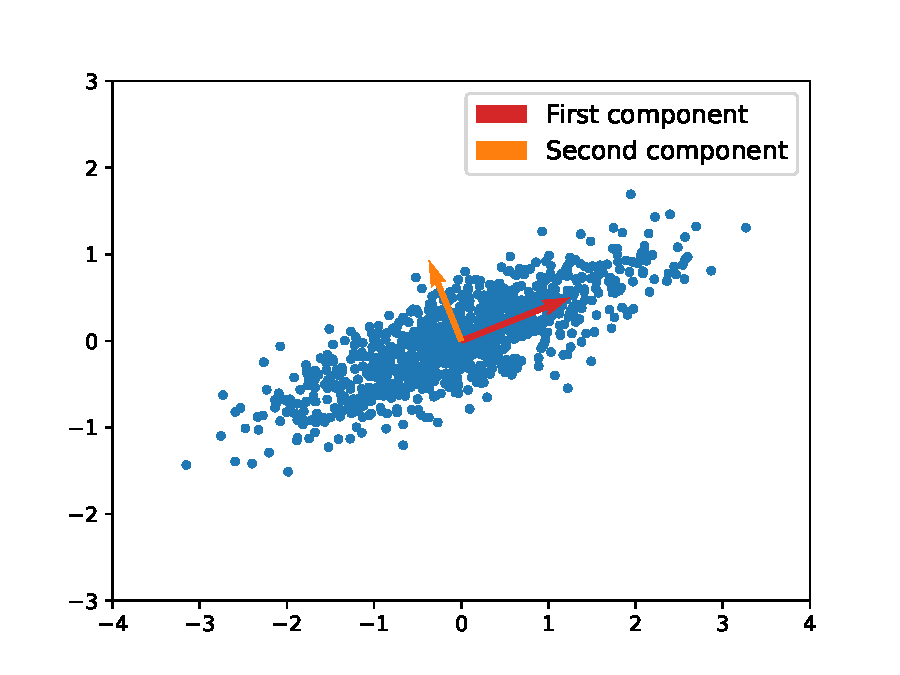
\includegraphics[width=0.255\textwidth]{before_pca.pdf}%
\label{fig_first_case}}
%\hfil
\subfloat[]{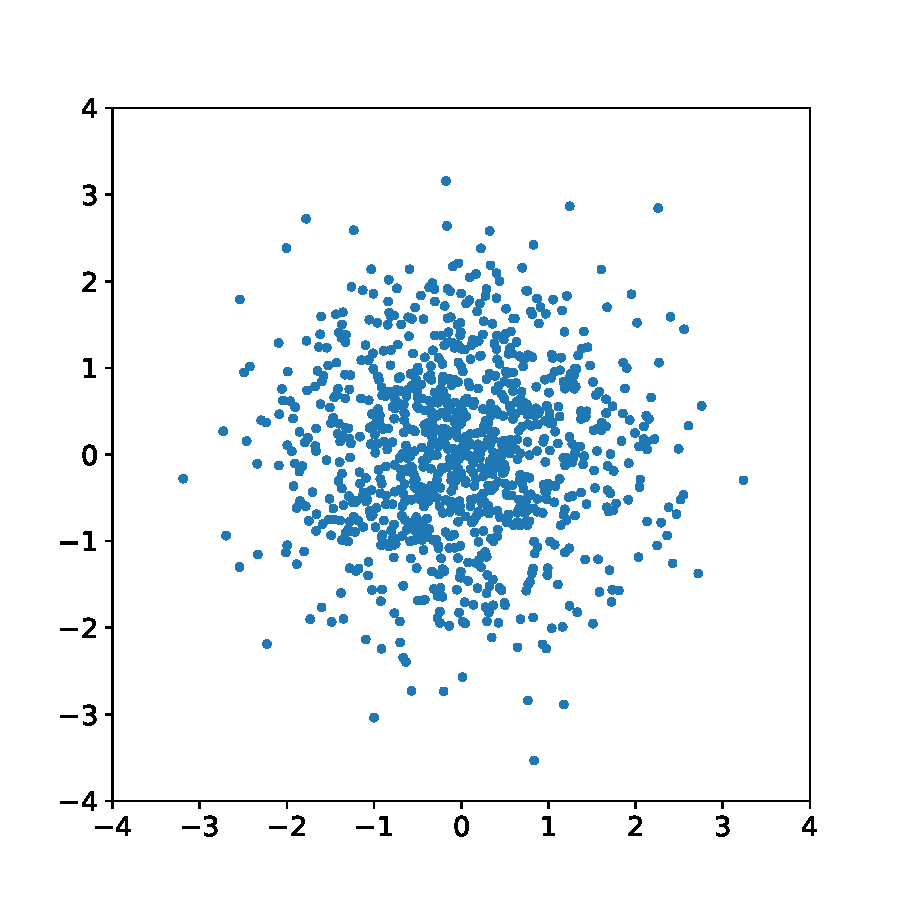
\includegraphics[width=0.195\textwidth]{after_pca.pdf}%
\label{fig_second_case}}
\caption{Example of PCA transform. Original data distribution is given by (a), where the two axes are highly correlated. (b) is the resultant distribution after applying Eq. (\ref{input_space}), where the correlation is removed.}
\label{PCA_outcome}
\end{figure}



\subsection{Choosing the Dynamics Representation}
We can use different representations of the dynamics $x_d$ in Eq. (\ref{dynamics_assumption}).
Apart from using $x$ and $y$ displacements (called displacement-based representation in this paper) as in RTE, another type of representation is investigated.
Since RTE uses periodic controllers, the robot will experience the same displacement and rotation during each period, and the execution should result in an arc.
Based on this analysis, we represent the dynamics as the tangential speed $v$, angular velocity $\omega$ and direction $\varphi$ (see Fig. \ref{arcs}). 
This design, called arc-based representation, considers the fact that the different dimensions of the dynamics are modelled by different GPs (hence are decoupled) in RTE.
This is not an ideal design since $x$ and $y$ are typically correlated.
In arc-based representation, these parameters are more decoupled and more consistent with real-world mechanics. 
Take a hexapod robot for example.
If the robot is carrying heavy payload and becomes slower, arc-based representation can easily model this distortion by reducing $v$ for all policies. However, for displacement-based representation, reduced speed will lead to decrease for positive displacements and increase for negative displacements.
In the case where the robot suffers damage in one of its legs, the side of the damaged leg will contribute lesser force, and the robot might move towards a different direction or rotate during the motion.
For arc-based representation, this can be modelled by adding a shift to the angular velocities and directions of the policies.
While it is a lot harder for the displacement-base representation, and $x$ and $y$ will become strongly correlated.
\begin{figure}[h]
\centering
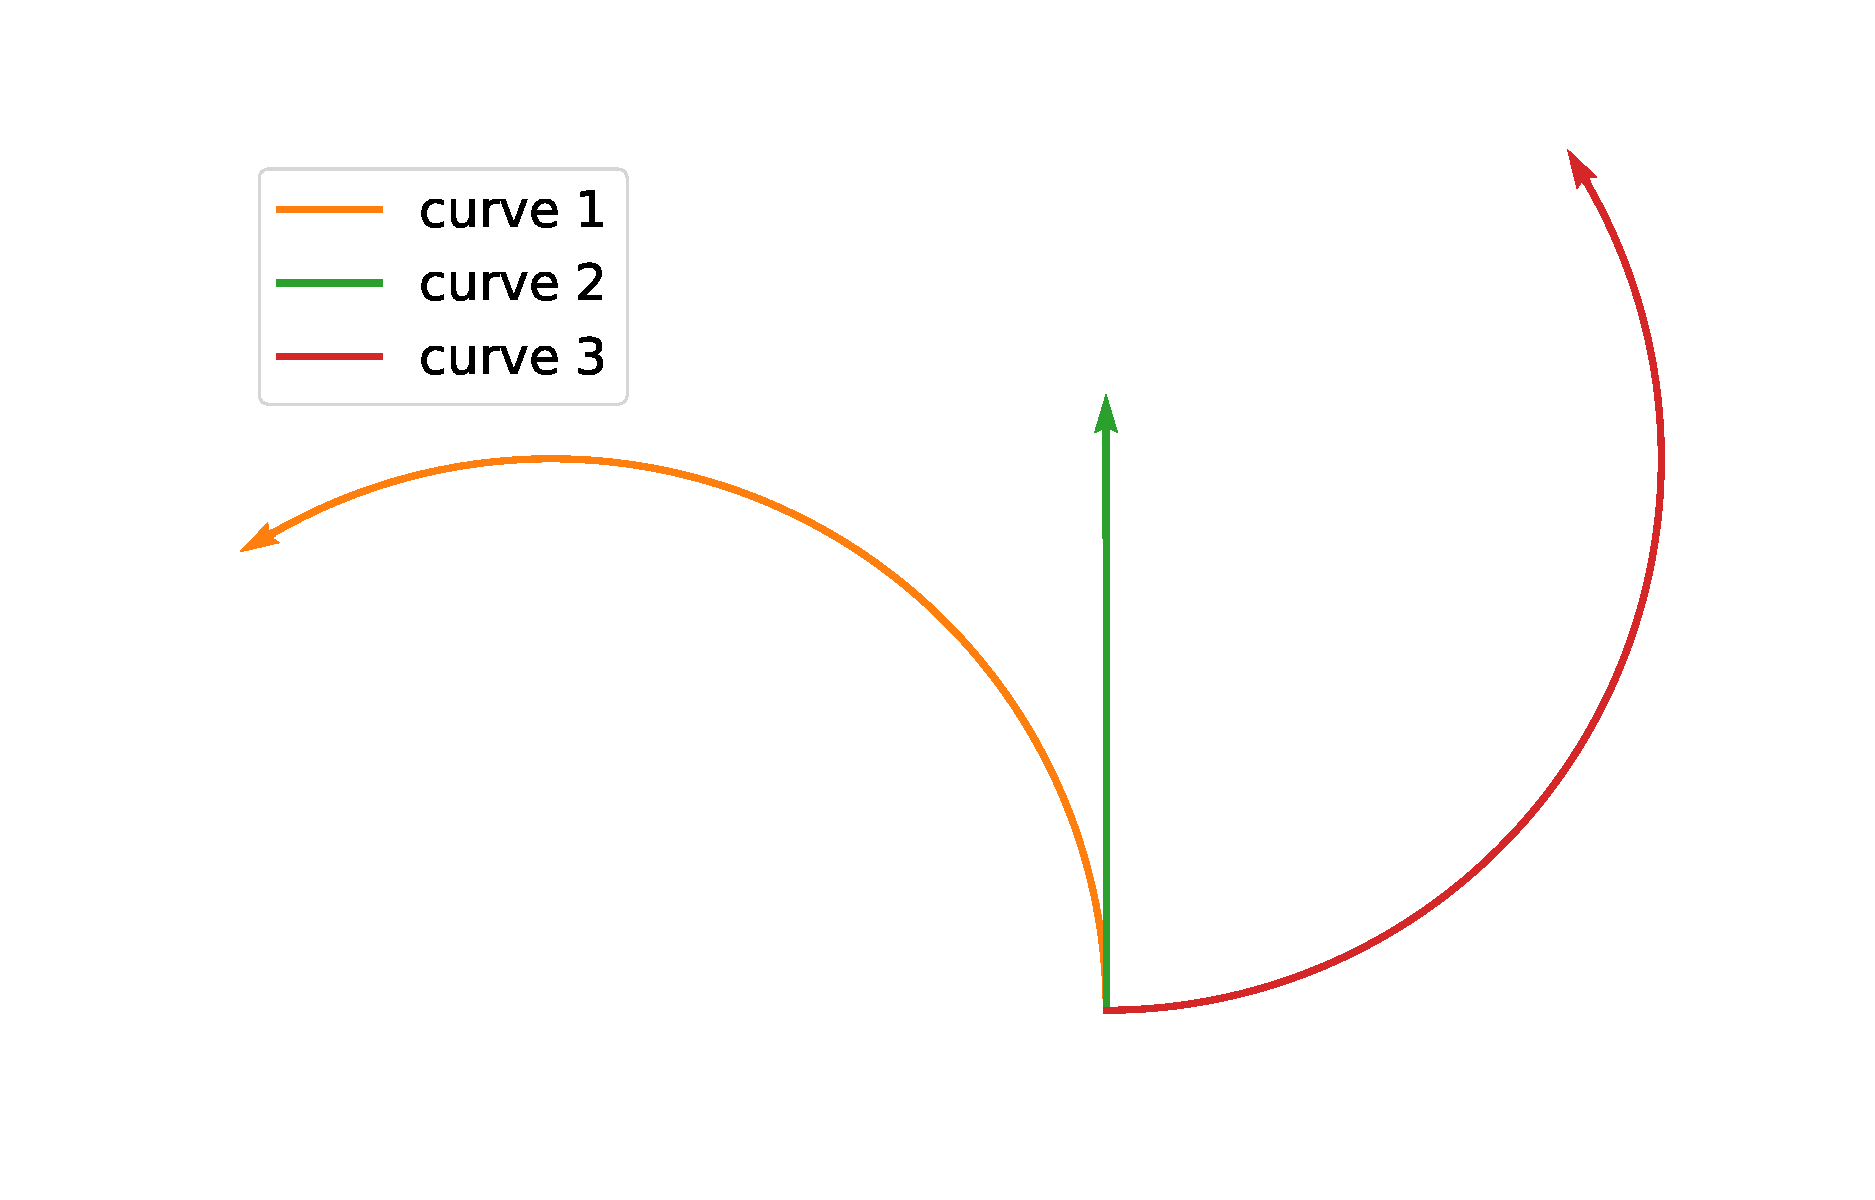
\includegraphics[width=0.45\textwidth]{example_curves.pdf}
\caption{Arc trajectories with different $v$, $\omega$ and $\varphi$. Curve 1 has $v=0.5$, $\omega = 30^\circ/s$ and $\varphi = 90^\circ$. Curve 2 has $v=0.25$, $\omega = 0$ and $\varphi = 90^\circ$.
Curve 3 shares the same $v$ and $\omega$ with curve 1 but having $\varphi = 0$.
All the curves are generated after 4 seconds of movement.
}
\label{arcs}
\end{figure}

To implement arc-based representation, we will need to get the three parameters $v$, $\omega$ and $\varphi$ from the trajectory. 
During the execution of each policy, we record the $x$ and $y$ positions of the robot as well as the time.
For a perfect arc, the points on the trajectory should obey the following equation:
\begin{equation}
(x - A)^2 + (y - B)^2 = A^2 + B^2
\label{circle_equation}
\end{equation}
Where $A$ and $B$ are the $x$ and $y$ coordinates of the center. In Eq. (\ref{circle_equation}) we have forced the curve to pass through the origin, which is the initial position of the robot.
Analytical estimate of the center can be provided by the classical circle fitting method called Kasa method \cite{Kasa_method}.
But this estimation is biased unless the points are symmetrically distributed across the entire circumference \cite{circle_fitting}.
While in most cases, the trajectory of the robot covers less than a quarter circle, and sometimes it is even a straight line.
Hence the Kasa method is not appropriate, and we aim to minimize the unbiased loss function: 
\begin{equation}
\mathcal{L} = 
\sum_{i=1}^N \left[
\sqrt{(x_i - A)^2 + (y_i - B)^2} - \sqrt{A^2 + B^2}
\right]^2
\label{circle_error}
\end{equation}
The optimal solution of this loss function is hard to obtain analytically, hence we use L-BFGS-B \cite{L-BFGS-B} optimization algorithm instead.
After finding the $A$ and $B$, we then get the angular change between each time step.
This is achieved by taking the cross product between the neighbouring points:
\begin{equation}
\begin{gathered}
\sin(\theta_2 - \theta_1) = \\
\frac{(x_1 - A)(y_2 - B)-(y_1 - B)(x_2 - A)}{
\sqrt{(x_1 - A)^2 + (y_1 - B)^2} \sqrt{(x_2 - A)^2 + (y_2 - B)^2}
}
\end{gathered}
\label{delta_theta}
\end{equation}
Because the $\sin (x)$ function is monotonically increasing between $[-\frac{\pi}{2}, \frac{\pi}{2}]$, we can determine the sign of the angular difference (positive for anti-clockwise).
Then, all three parameters can be calculated:
\begin{equation}
\begin{gathered}
\omega = \frac{
\sum_{i=1}^{N-1} \Delta \theta_i \Delta t_i}{
\sum_{i=1}^{N-1} \Delta t_i^2}
\text{ , }
v = \sqrt{A^2 \omega^2 + B^2 \omega^2}
\\
\text{and \,}
\varphi = \operatorname{atan2}(-B, -A) + 
\begin{cases} 
\frac{\pi}{2} & \text{if } \omega > 0 \\
-\frac{\pi}{2} & \text{if } \omega < 0 
\end{cases}
\end{gathered}
\label{all_three_parameters}
\end{equation}
%
To correctly determine the direction, Eq. (\ref{all_three_parameters}) suggests that we need to make sure the $\omega$ is never zero even for a straight line.
In practice, we can achieve this by giving an upper bound to the absolute values of the center coordinates $A$ and $B$, which is the reason we use L-BFGS-B optimization algorithm.
This ensures that the center will not tend to infinity, and hence the absolute value of $\omega$ will always be positive for any trajectory. 
In the extreme case where the robot remains stationary, we must still assign a non-zero value to the $\omega$ to avoid zero division in further calculations, but the direction $\varphi$ can take any value.


One thing to notice is that while the measurement of tangential speed $v$ is always accurate, the measurement of $\omega$ and $\varphi$ can be very noisy in some cases.
For example, if the robot barely moves, the trajectory will be dominated by noise.
Hence the angular velocity $\omega$ and the direction $\varphi$ will become very noisy although they barely make any difference.
While in the case when the robot is travelling fast, $\omega$ and $\varphi$ will be very important and will have accurate measurements as well.
Hence, when modelling the arc-based dynamics representation with GP, it is reasonable to give different noises for different parameters in different trajectories.


To achieve this, we know that the robot coordinates can be regarded as a superposition of the ground truth and a random noise.
Our parameters calculated using Eq. (\ref{all_three_parameters}) correspond to the best-fit arc, and are also affected by this noise.
If we only focus on the final position after executing a policy, and we assume that the random noise only depends on the environment but not the policies, we can write:
%
\begin{equation}
\begin{gathered}
\sigma_{\hat{x}}^2 + \sigma_{\hat{y}}^2 = 2 \sigma_{\epsilon}^2
\end{gathered}
\label{summed_variance}
\end{equation}
%
where we have assumed the same noise variance $\sigma_{\epsilon}^2$ on both $x$ and $y$ axis.
The $\hat{x}$ and $\hat{y}$ denote the final coordinates given by the arc, where:
\begin{equation}
\begin{gathered}
\hat{x}(t | v, \omega, \varphi) 
%= \int_0^t v \cdot \cos(\varphi + \omega \tau) d\tau 
= \frac{v}{w} \left[ \sin(\omega t + \varphi) - \sin(\varphi) \right]
\\
\hat{y}(t | v, \omega, \varphi) 
%= \int_0^t v \cdot \sin(\varphi + \omega \tau) d\tau 
= \frac{v}{w} \left[ \cos(\varphi) - \cos(\omega t + \varphi) \right]
\end{gathered}
\label{position_from_arc}
\end{equation}
%
The term $\sigma_{\hat{x}}^2$ and $\sigma_{\hat{y}}^2$ in Eq. (\ref{summed_variance}) are related to the uncertainties in our measurement of $v$, $\omega$ and $\varphi$.
To study this relation, we model the error propagation with linear approximation, where the error of the random variable $f(x, y, z)$ is given by \cite{error_analysis}:
\begin{equation}
\begin{gathered}
\sigma_f^2 \approx
\frac{\partial f}{\partial x}^2 \sigma_x^2
+ \frac{\partial f}{\partial y}^2 \sigma_y^2
+ \frac{\partial f}{\partial z}^2 \sigma_z^2
\end{gathered}
\label{error_prapagation}
\end{equation}
Eq. (\ref{error_prapagation}) requires the random variables $x$, $y$ and $z$ be independent, which is consistent with our design.
Combining the above three equations, we will get:
\begin{equation}
\begin{gathered}
2\sigma_{\epsilon}^2 \approx 
\left(
 \frac{\partial \hat{x}}{\partial v}^2
 + \frac{\partial \hat{y}}{\partial v}^2
\right) \sigma_v^2 
\\ +
\left(
\frac{\partial \hat{x}}{\partial \omega}^2
+
\frac{\partial \hat{y}}{\partial \omega}^2
\right) \sigma_{\omega}^2 
 +
\left(
\frac{\partial \hat{x}}{\partial \varphi}^2
+ 
\frac{\partial \hat{y}}{\partial \varphi}^2
\right) \sigma_{\varphi}^2
\end{gathered}
\label{combined_error_relation}
\end{equation}
Since the LHS of the Eq. (\ref{combined_error_relation}) is invariant to the policies, it is reasonable to assume that:
\begin{equation}
\begin{gathered}
\sigma_v^2 \propto
\frac{1}{
\frac{\partial \hat{x}}{\partial v}^2 
+ \frac{\partial \hat{y}}{\partial v}^2 + \varepsilon_v}
\\
\sigma_{\omega}^2 \propto
\frac{1}{
\frac{\partial \hat{x}}{\partial \omega}^2
+
\frac{\partial \hat{y}}{\partial \omega}^2 + \varepsilon_{\omega}} 
\\
\sigma_{\varphi}^2 \propto
\frac{1}{
\frac{\partial \hat{x}}{\partial \varphi}^2
+ 
\frac{\partial \hat{y}}{\partial \varphi}^2 + \varepsilon_{\varphi}} 
\end{gathered}
\label{noises_for_v_w_phi}
\end{equation}
where a positive small constant is added at the each denominator for numerical stability.
This result is very reasonable as higher dependency on the parameter leads to smaller noise.
Although Eq. (\ref{noises_for_v_w_phi}) doesn't give the exact value for the noises, it provides a method to calculate relative noises between different policies in the same environment.



\subsection{Clustering the Dynamics with Dirichlet Processes}
So far, we have determined the basis for our linear prior mean function, the input space, different representations of dynamics as well as the way to calculate relative noises.
To cluster the historical data with DP, we still need the prior distribution $H$ for the detailed parameters for the GPs. 
These parameters typically refer to the weights $\bm{w}$ for the linear mean function.
But in our case, we also allowed the kernels to be non-stationary for higher flexibility.
This design is to incorporate the possibility that the Bayesian inference in the input space could be different in each environment.
Hence, we also need to determine the prior distribution for the length scales $\bm{l}$, the prior variance $\alpha_0$, and the noises variance $\sigma_{n}^2$.
Such distribution is hard to give since we have little prior knowledge.
Even if we could give a perfect prior distribution, the integrals in Eq. (\ref{integral_1}) and Eq. (\ref{integral_2}) are intractable since we allowed the kernel parameters to be variables.


The solution is to use Monte Carlo sampling combined with a trick called posterior convergence estimate.
We can see that these parameters are all related to the environment.
The Monte Carlo sampling is to collect a sample of these environment-related parameters from the simulation as our prior distribution $H$.
To do this, we first randomize the simulation settings to get a sample of simulated environments.
We then collect a sufficient amount (e.g. 64) of interaction data from each environment and find the detailed parameters using maximum likelihood estimate (MLE):
\begin{equation}
\bm{\theta}^* = 
\arg \max_{\bm{\theta}} \, p(\bm{y}|\bm{\theta})
= \arg \min_{\bm{\theta}} \, -\log p(\bm{y}|\bm{\theta})
\label{MLE}
\end{equation}
The probabilistic model in our case is a product of GPs over the dimensions, and $p(\bm{y}|\bm{\theta})$ can be calculated from Eq. (\ref{multi_normal}):
\begin{equation}
\begin{gathered}
-\log p(\bm{y}|\bm{\theta}) = \sum_{d} -\log p(\bm{x}_{d}|\bm{\theta}_d)
\\
= \frac{1}{2} \sum_{d}
(\bm{x}_{ d} - \bm{\mu}_{\bm{\theta}_d})^T \bm{\Sigma^{-1}}_{\bm{\theta}_d} (\bm{x}_{d} - \bm{\mu}_{\bm{\theta}_d})
\\ + \sum_{ d} \left[ \frac{N}{2}\log(2\pi) 
+ \log \det(\bm{\Sigma}_{ \bm{\theta}_d}) \right]
\end{gathered}
\label{nll}
\end{equation}
where the weights $\bm{w}_d$ are encoded in $\bm{\mu}_{\bm{\theta}_d}$, and the rest of the parameters are encoded in $\bm{\Sigma}_{\bm{\theta}_d}$.
It is worth noting that the noise $\sigma_n^2$ in displacement-based representation is the same for all policies; while in arc-based representation, Eq. (\ref{covariance_matrix}) needs to be modified:
\begin{equation}
\bm{\Sigma} = \bm{K}(\bm{x_{1:N}}, \bm{x_{1:N}}) + \sigma_{n}^2 \bm{D}
\label{modified_covariance_matrix}
\end{equation}
where matrix $\bm{D}$ is a diagonalized matrix with entries calculated according to Eq. (\ref{noises_for_v_w_phi}).
The optimal solution of Eq. (\ref{MLE}) can be obtained using optimization algorithms like L-BFGS-B. 
The Monte Carlo sampling seems computationally expensive. But note that the sample amount for each environment is small and invariant to the size of the repertoire.
Hence it is much cheaper to do than finding the basis for the prior mean function, where we need to evaluate all the policies in several environments.
Since we have used Monte Carlo sampling to represent the prior, the integrals in Eq. (\ref{integral_2}) and Eq. (\ref{integral_1}) now become averages over finite number of terms:
\begin{equation}
\begin{gathered}
p(y_i|c_i, \bm{y}_{-i}, \bm{c}_{-i}) = 
\sum_{l=1}^L p(y_i|\bm{\theta}^{(l)})
p(\bm{\theta}^{(l)}|c_i, \bm{y}_{-i}, \bm{c}_{-i})
\\
p(y_i|c_i \neq j \, \text{for any} \, n_j \neq 0) = 
\frac{1}{L} \sum_{l=1}^L p(y_i|\bm{\theta}^{(l)})
\end{gathered}
\label{MC_prior_integral}
\end{equation}
Where the posterior distribution is:
\begin{equation}
p(\bm{\theta}^{(j)}|c_i, \bm{y}_{-i}, \bm{c}_{-i}) = 
\frac{
\prod_{c_k=c_i, k \neq i} p(y_k|\bm{\theta}^{(j)})}
{\sum_{l=1}^L \prod_{c_k=c_i, k \neq i} p(y_k|\bm{\theta}^{(l)})}
\label{MC_posterior}
\end{equation}
In practice, it is much easier and numerically stable to work with logarithm likelihoods as in Eq. (\ref{nll}), as the direct product of likelihoods will very likely lead to overflow.


Although the integrals are now made tractable, this method has two fatal shortages.
First, the Monte Carlo sampling only provides limited precision of the parameters.
As each cluster grow larger, Eq. (\ref{MC_posterior}) implies that the set of parameters that is closest to the ground truth will eventually make up 100\% of the posterior weight.
Hence, the number of clusters will not exceed the amount of sampled priors. 
Second and more importantly, the prior collection is made in simulation, which ensures no extrapolation to the real-world dynamics.
To solve these two shortages, we introduce a trick called posterior convergence estimate.
As a cluster gathers more data, the posterior distribution of its parameters will become narrower and more centred closer to the ground truth (see Fig \ref{posterior_convergence}).
When the cluster size is large, we can safely assume that the posterior becomes a sharp spike.
Hence, we may treat it as a Dirac delta distribution, and Eq. (\ref{integral_1}) becomes:
\begin{equation}
\begin{gathered}
p(y_i|c_i, \bm{y}_{-i}, \bm{c}_{-i}) \approx 
\int p(y_i|\bm{\theta})
\delta (\bm{\theta} - \bm{\theta}^*)
d\bm{\theta}
\\
= p(y_i|\bm{\theta}^*)
\end{gathered}
\label{posterior_convergence_estimate}
\end{equation}
This is called posterior convergence estimate, and the center of this Dirac delta is located using MAP. 
This means we refit the parameters for large clusters (with data size above a threshold, e.g. 30) as their posterior.
This design is to leverage the fact that for small clusters, their posteriors haven't converged and spread across the parameter space.
Hence the integrals can be efficiently approximated by Eq. (\ref{MC_prior_integral}).
While for large clusters, their posterior cannot be well represented by any prior sample, so we allow them to determine the best parameters based on their data.
The only thing that such prior should satisfy is that it covers a variety of possible cases.
Thus, the use of Monte Carlo sampling for the prior acts like a guide for smaller clusters, but neither the coverage of parameters nor the number of clusters is constrained by the sampled prior. 
\begin{figure}[h]
\centering
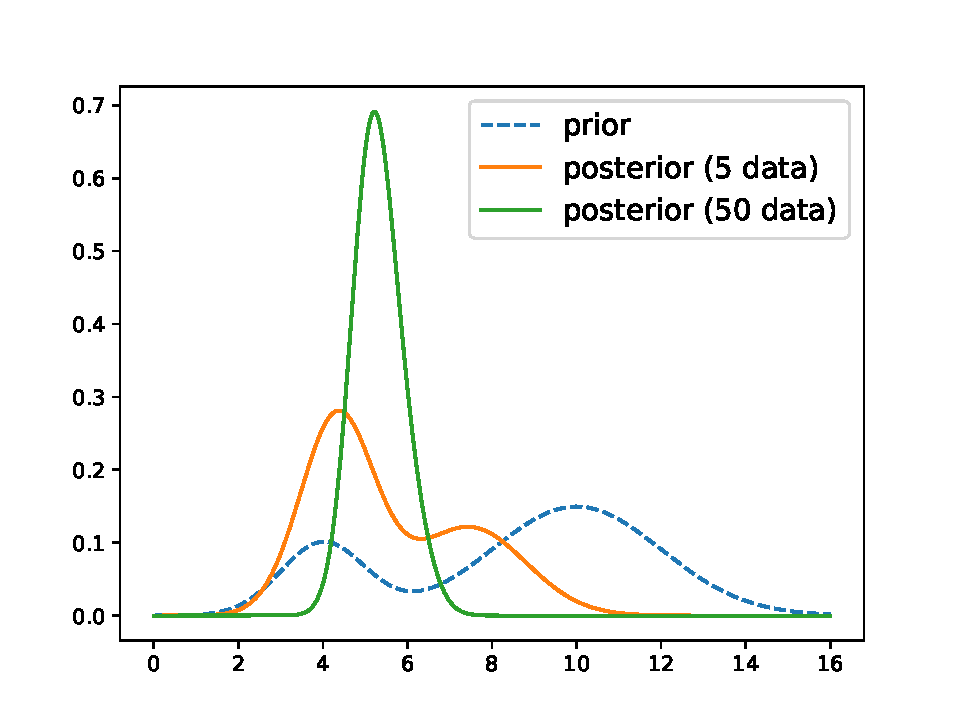
\includegraphics[width=0.45\textwidth]{posterior_convergence.pdf}
\caption{Example of the convergence of parameter posterior in DPMM.
Data are sampled from a infinite mixture of Gaussians, where the variance is fixed at 4, and the mean is given by a Gaussian mixture as the prior.
As the cluster grows larger, the posterior of the mean becomes more narrowed and centred at the ground truth (5.5).
}
\label{posterior_convergence}
\end{figure}

Because we have no access to the analytical form of the prior to do MAP, we can use MLE instead (for large data size, MLE and MAP gives similar results).
Hence, during Gibbs sampling, the likelihood of an episode belonging to a large cluster is calculated according to Eq. (\ref{posterior_convergence_estimate}), while the likelihood of belonging to a small cluster is calculated using the first equation in Eq. (\ref{MC_prior_integral}).
As mentioned previously, the episode needs to be removed from its current cluster which will affect the posterior when calculating the likelihood of this episode staying in its current cluster.
For small cluster, we can easily recalculate the posterior using Eq. (\ref{MC_posterior}).
For large cluster, if the data size is still large enough without this episode, the parameter $\bm{\theta}^*$ needs to refitted with this episode removed.
If the data size is no longer large enough without this episode, the posterior is calculated in the same way as a small cluster.
After each resample step, we also need to refit the parameters for large clusters if any change is made.
Be aware that the subscript $i$ in Eq. (\ref{MC_prior_integral}), Eq. (\ref{MC_posterior}) and Eq. (\ref{posterior_convergence_estimate}) refers to each episode instead of each individual interaction data. 
Similarly, the $N$ and $n_j$ in Eq. (\ref{indicator_posterior_3}) correspond to the number of episodes instead of the amount of data.


In practice, refitting all the parameters in each step of Gibbs sampling could lead to performance issues as the Gibbs sampling cannot be paralleled.
It is much cheaper to just refit the weights for the prior mean function as they are most important can be obtained analytically.
Hence, for a large cluster, we use the most likely kernel in the Monte Carlo sampled prior and calculate the best fitting weights using:
\begin{equation}
\bm{w}_d^* = \left(\sum_{i=1}^n
\bm{X}_i^T \bm{\Sigma}_{i, \bm{\theta}_d}^{-1} \bm{X}_i
\right)^{-1} \sum_{i=1}^n \left( \bm{X}^T_i \bm{\Sigma}_{i, \bm{\theta}_d}^{-1} \Delta \bm{x}_{i, d} \right)
\label{refitted_weights}
\end{equation}
This is the formula we use to determine the most suitable prior for each cluster.
The summation is made over all the episodes in the cluster.
$\Delta \bm{x}_{i, d}$ is the real-world distortions of the $i^{\text{th}}$ episode.
$\bm{X}_i$ is the coordinate matrix of this episode, where each row gives the coordinates of the policy corresponding to each interaction.
The covariance matrix $\bm{\Sigma}_{i, \bm{\theta}_d}$ is generated using the most likely kernel.

To sum up, the complete algorithm for conducting DP clustering is presented in the pseudo code below:
\begin{algorithm}
\caption{DP Clustering}
\begin{algorithmic}
\STATE \textbf{procedure} DP Clustering
\STATE $\mathcal{R} \leftarrow $ MAP{\_}Elites() \COMMENT{Generate the repertoire}
\STATE $\bm{X} \leftarrow \emptyset$ \COMMENT{Initialize collected distortions}
\FOR{$\bm{i} = 1 \rightarrow G$}
\STATE $\varepsilon \leftarrow$ random{\_}simulation{\_}settings()
\STATE $\Delta \bm{x}_{1:D} \leftarrow $ evaluate{\_}repertoire($\mathcal{R}$, $\varepsilon$)
\STATE $\bm{X}$.append($\Delta \bm{x}_{1:D}$)
\ENDFOR
\STATE $\bm{X} \leftarrow$ SVD($\bm{X}$) \COMMENT{Reduce the dimensionality via SVD}
\STATE $\bm{X} \leftarrow$ PCA($\bm{X}$) \COMMENT{Convert into input space via PCA}
\STATE 

\STATE $H \leftarrow \emptyset$ \COMMENT{Initialize Monte Carlo sampled priors}
\FOR{$\bm{i} = 1 \rightarrow N$}
\STATE $\varepsilon\leftarrow$ random{\_}simulation{\_}settings()
\STATE $\mathcal{D} \leftarrow \emptyset$ \COMMENT{Initialize dataset}
\FOR{$\bm{j} = 1 \rightarrow M$} 
\STATE $\Theta \leftarrow$ evaluate{\_}random{\_}policy()
\STATE $\mathcal{D}$.append($\Theta$)
\ENDFOR
\STATE $\bm{\theta} \leftarrow$ MLE($\mathcal{D}$) \COMMENT{Find the parameters with MLE}
\STATE $H$.append($\bm{\theta}$)
\ENDFOR
\STATE \COMMENT{Gibbs sampling}


\STATE $\xi^{*} \leftarrow -\infty$ \COMMENT{Initialize highest likelihood}
\STATE $\mathcal{C} \leftarrow$ initialize{\_}cluster{\_}assignment() 
\FOR{$\bm{i} = 1 \rightarrow T$} 
\STATE $\mathcal{C}$, $\xi$ $\leftarrow$ Gibbs{\_}sampling{\_}sweep($\mathcal{C}$, $H$)
\IF{$\xi > \xi^{*}$}
\STATE $\xi^{*} \leftarrow \xi$
\STATE $\mathcal{C}^{*} \leftarrow \mathcal{C}$ \COMMENT{Record the best result}
\ENDIF
\ENDFOR
\RETURN $\mathcal{C}^{*}$ 
\end{algorithmic}
\label{DP_clustering}
\end{algorithm}
In our implementation, we modelled the clustering and online-adaptation to be made in two separated systems.
The DP clustering of historical data is conducted in the archive management system, which would typically be a cloud server where expensive data processing is available.
After having found the clusters, the results are saved as an adaptation system to be used (downloaded) by individual robots.
The adaptation system is independent from the archive, and we are free to make simplifications for embedded systems.





\subsection{Learning the Dynamics Online}
In theory, the dynamics is modelled with an infinite mixture of GPs, where the GP parameters follow a finite mixture of distributions:
\begin{equation}
p(\bm{\theta}) = \sum_j \frac{n_j}{n + \alpha} p(\bm{\theta}|c=j) 
+ \frac{\alpha}{n + \alpha} H(\bm{\theta})
\label{trained_mixture_model}
\end{equation}
where the summation is made over the clusters containing at least one episode, and $p(\bm{\theta}|c=j)$ denotes the posterior of parameters for the $j^{\text{th}}$ cluster.
The last term results from the important property of DPMM that there is always a non-zero probability that we will get a new cluster (face a new situation).
Each instance of $\bm{\theta}$ sampled from $p(\bm{\theta})$ is a certain configuration of parameters of GP, and the learned distortion is integrated over the posterior of $\bm{\theta}$ conditioned on the real-world interactions collected online:
\begin{equation}
\begin{gathered}
p(x^*_d|\bm{x}_{1:N}) 
\\
= \sum_j p(c=j| \bm{x}_{1:N}) \int p(x^*_d|\bm{\theta}, \bm{x}_{1:N})p(\bm{\theta}|c=j, \bm{x}_{1:N}) d\bm{\theta} 
\\
+ p(c \neq j, \forall j|\bm{x}_{1:N}) \int p(x^*_d|\bm{\theta}, \bm{x}_{1:N}) p(\bm{\theta} | \bm{x}_{1:N}) d\bm{\theta}
\end{gathered}
\label{MGP_posterior}
\end{equation}
where the indicator probabilities are given by:
\begin{equation}
\begin{gathered}
p(c=j| \bm{x}_{1:N}) 
= \frac{n_j \cdot p(\bm{x}_{1:N}|c=j)
}{Z}
\\ 
p(c \neq j, \forall j| \bm{x}_{1:N})
= \frac{\alpha \cdot p(\bm{x}_{1:N}|c \neq j, \forall j)
}{Z}
\end{gathered}
\label{MGP_indicator}
\end{equation}
where $\bm{x}_{1:N}$ stands for the collected ($N$ number of) interaction data during deployment.


In practice, approximations have to be made since Eq. (\ref{MGP_indicator}) requires calculating multiple complicated and intractable integrals over the posteriors. 
Fortunately, if we have applied posterior convergence estimate for $p(\bm{\theta}|c=j)$, we will have:
\begin{equation}
\begin{gathered}
\int p(x^*_d|\bm{\theta}, \bm{x}_{1:N})p(\bm{\theta}|c=j, \bm{x}_{1:N}) d\bm{\theta} \approx p(x^*_d|\bm{\theta}^*_j, \bm{x}_{1:N})
\\
\text{and } p(\bm{x}_{1:N}|c=j) \approx p(\bm{x}_{1:N}|\bm{\theta}^*_j)
\end{gathered}
\label{posterior_convergence_simplification}
\end{equation}
where $\bm{\theta}^*_j$ denotes the optimal parameters for the cluster $j$.
Hence for simplicity, we can apply posterior convergence estimate for all the clusters we have found.
For the clusters that are not large enough to refit the parameters, we will just use the parameters of the most likely prior sample.
As for clusters that are very small, this might be inappropriate, and we can simply discard them from the adaptation system.
Apart from the clusters we have found, DPMM also gives an extra term that corresponds to the case of a new cluster (facing a new situation).
One of the solutions is to use Monte Carlo sampling and replace the last integrals in Eq. (\ref{MGP_posterior}) and Eq. (\ref{MGP_indicator}) by the summations over a large number of samples.
In this paper, we take a very simple alternative by using RTE to incorporate this new situation.
Although RTE is not optimized for any environment, it offers a satisfying baseline performance in all situations.
The non-zero probability of encountering new cases secured by DP and the use of RTE ensures that we can always adapt well to new situations and hence will never over-fit to the training data.
Combined with Eq. (\ref{posterior_convergence_simplification}), the predicted distortion becomes a finite mixture of GPs:
\begin{equation}
\begin{gathered}
p(x^*_d|\bm{x}_{1:N}) 
= \sum_j p(c=j| \bm{x}_{1:N}) p(x^*_d|\bm{\theta}^*_j, \bm{x}_{1:N})
\\
+ \,\, p(c \neq j, \forall j|\bm{x}_{1:N})  p(x^*_d|\bm{x}_{1:N}, \text{RTE})
\end{gathered}
\label{simplified_distortion}
\end{equation}
where the indicator probabilities are:
\begin{equation}
\begin{gathered}
p(c=j| \bm{x}_{1:N}) 
= \frac{n_j \cdot p(\bm{x}_{1:N}|\bm{\theta}^*_j)
}{Z}
\\ 
p(c \neq j, \forall j| \bm{x}_{1:N})
= \frac{\alpha \cdot p(\bm{x}_{1:N}|\text{RTE})
}{Z}
\\ \text{where }
Z = \sum_k n_k \cdot p(\bm{x}_{1:N}|\bm{\theta}^*_k) + \alpha \cdot p(\bm{x}_{1:N}|\text{RTE})
\end{gathered}
\label{simplified_indicator}
\end{equation}
This is much cheaper to evaluate, and the performance shouldn't suffer too much from the simplifications we made.


In contrast to RTE, our online learning of the dynamics consists of two levels.
The first level is to use the real-world data to figure out the situation that the robot is in.
This will affect the probabilities for each GP (with the corresponding prior) to be employed for prediction making.
Considering the dynamics can be distinct for different environments, the robot should be able to quickly figure out its current situation.
Since the prior for each situation that can give estimation of the dynamics without further data, our method should be able to provide fast online learning of the real-world dynamics with much higher data-efficiency than RTE.
The second level is to learn the residual dynamics, which is the part of the distortion failed to be captured by the prior mean, using the kernels optimized for each situation.
The final prediction of dynamics given by Eq. (\ref{simplified_distortion}) is a mixture of Gaussians.
The mean and variance for each mixture component are calculated using Eq. (\ref{GP_posterior}), and the mixture weights are the probabilities of being in each situation, namely the indicator probability given by Eq. (\ref{simplified_indicator}).
This learned dynamics can then be used by the robot to correct its motion accordingly, hence performing model-based online adaptation.





%To formulate the problem clearly, we are aiming to leverage the collaboratively collected real-world interactions to assist a robot deployed in an unknown environment to quickly adapt and complete its task.
%We are provided with some episodes (each task-solving process corresponds to an episode of interaction data) of real-world interactions collected by several robots deployed in an unknown distribution of environments.
%The most intuitive idea is to label these historical data with their sources (like collected from grass terrain, collected with left leg broken, etc.) and build a simple database in the cloud server. 
%During the adaptation, the robot examines the current environment and uploads the result to the database server. The server then identifies the most similar environment recorded in the database and let the robot download the corresponding data to assist the its adaptation.
%However, accurately measuring and describing the environment can be expensive and difficult. It is also hard to determine whether a previously encountered environment shares similar dynamics with the current one even if we have accurate descriptions for them.
%In the case we do know that some historical data come from exactly the same environment as the current one, these data might be insufficient in quantity to assist the current task.
%Hence, it is reasonable to group the episodes resulting from similar dynamics into clusters, ensuring having enough data for analysis.
%We will assume that we don’t have access to any information of the environment and aim to conduct clustering only according to the dynamics. 






\section{Experiment Design}



\subsection{Robot Setup}
To evaluate our methodology, experiment is conducted on the Ant robot in PyBullet simulation \cite{PyBullet} (see Fig \ref{Ant_robot}). 
This robot has 8 degrees of freedom (2 for each leg) corresponding to 8 motors powering its motion.
Note that the joints connecting the body and each leg can only rotate horizontally, meaning that the four thighs (the part of each leg directly attached to the body) are always on the same plane.
Hence, the Ant robot cannot lift up its leg to walk like real animals.
The motors employ PID positional control, where the torque is given by:
\begin{equation}
\tau = K_p \theta_e + K_i \int \theta_e(t) dt + K_d \frac{d \theta_e}{dt}
\label{PID}
\end{equation}
where $\theta_e = \theta_t - \theta$ ($\theta_t$ is the positional target).
In PyBullet, the maximum torque is $\pm 1$. 
For the motors on the body, $K_p$ is set to be 1.43 and $K_d$ is set to be 0.072.
For the motors on the knees, $K_p$ is 1.637 and $K_d$ is 0.082.
For all motors, $K_i$ is set to zero for simplicity. 
\begin{figure}[h]
\centering
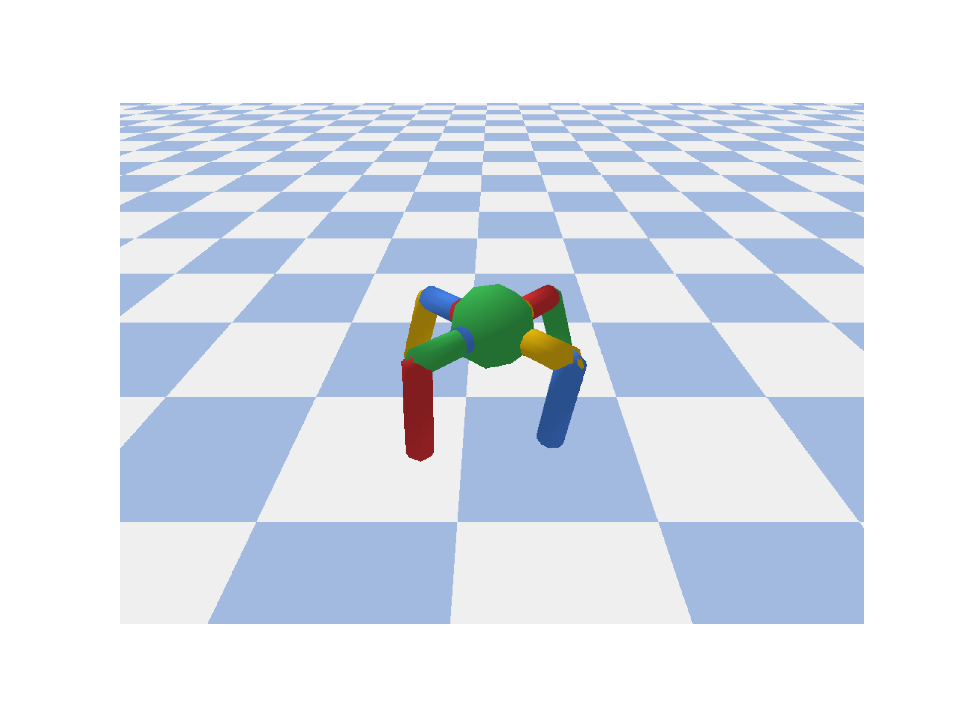
\includegraphics[width=0.45\textwidth]{intact_robot.pdf}
\caption{The Ant robot in PyBullet simulation. 
The four motors mounted on the body can rotate from $-40^{\circ}$ to $40^{\circ}$. The knee flexion angle for each leg ranges from 
$30^{\circ}$ to $100^{\circ}$.
}
\label{Ant_robot}
\end{figure}


Like in RTE, we use a periodic controller for the robot.
The period is set to 1 second, which corresponds to 100 time-steps in simulation.
The targets within each period is parametrized in the same way as in \cite{cully2015robots}.
The target of each motor is a smoothed squared wave (see Fig \ref{targets}) governed by three parameters: amplitude $\alpha$, phase $\phi$ and duty cycle $\tau$.
All the three parameters range from 0 to 1.
The duty cycle stands for the proportion of time in one period that the squared wave is in its high state.
This squared wave is then smoothed by a Gaussian kernel to remove rapid changes.
In each time-step of the simulation, we give each motor the corresponding positional target, which will then be converted into torques via PID.
Thus, each controller is parametrized by a vector of 24 dimensions, which is hence defined to be the genotype of this controller.
%
%
\begin{figure}[H]
\centering
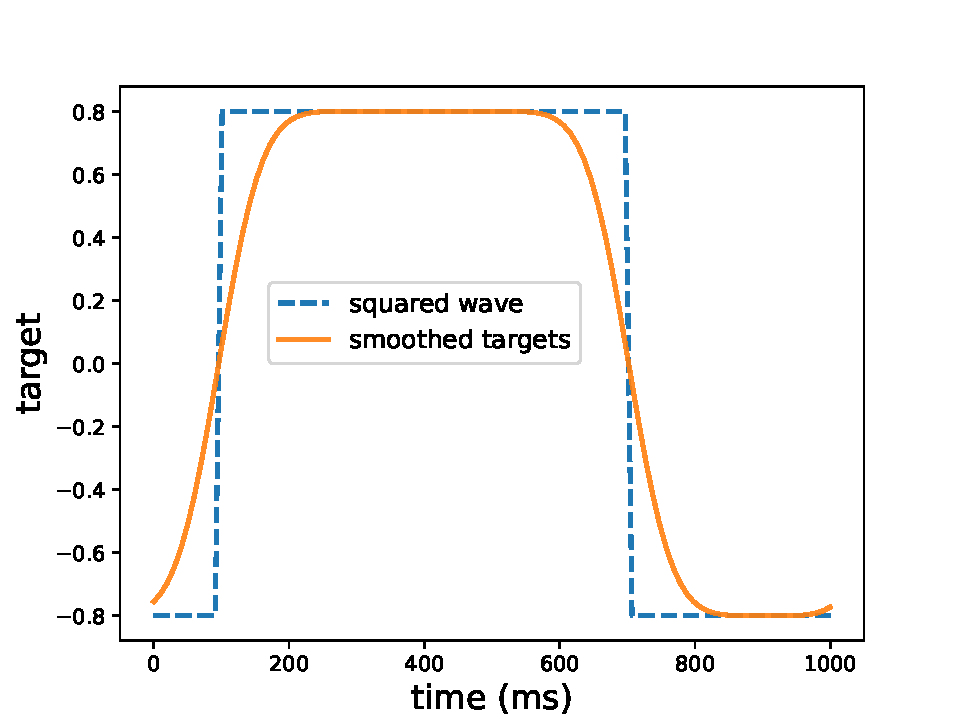
\includegraphics[width=0.45\textwidth]{targets.pdf}
\caption{The periodic motor targets corresponding to $\alpha = 0.8$, $\phi=100$ ms and $\tau=0.6$.
The squared wave is smoothed by a Gaussian kernel with $\sigma = 100$ ms.
}
\label{targets}
\end{figure}


In this paper, we consider three sources of distortions: friction, payload and damages to the legs of the robot.
To collect the distortions as the basis for the prior mean function, we need to model these sources in simulation.
Different frictions can be easily achieved by changing the simulation settings.
Leg damages are modelled by giving a fixed positional target to the motor mounted on the knee.
This fixed target overwrites the command of the controller, so that the damaged leg is always in the upper position (see Fig \ref{damaged_robot}).
However, for unknown reasons, changing the mass of the robot do not affect the dynamics in simulation. 
Hence, we take an alternative approach by discounting the torque to model the payload.
%
%
\begin{figure}[h]
\centering
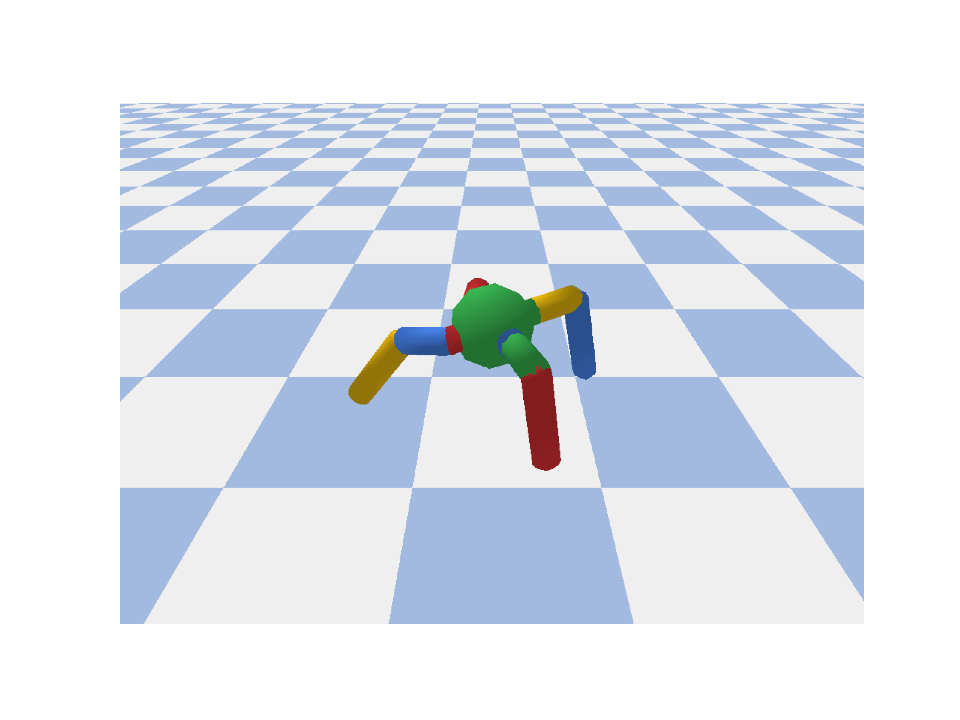
\includegraphics[width=0.45\textwidth]{damaged_robot.pdf}
\caption{The robot walking with one leg (left blue-yellow leg) damaged.
The knee flexion angle of this leg is fixed at $30^{\circ}$ to reduce contact with the ground.
}
\label{damaged_robot}
\end{figure}




\subsection{Generating the Repertoire with MAP-Elites}
To implement MAP-Elites, the task space for our robot is defined to be its 2D displacement, spanning from -4.8 to 4.8 on both the $x$ and $y$ axes. 
This continuous space is then discretized into a $32 \times 32$ grid, yielding a resolution of 0.3 unit per cell.
In each iteration of MAP-Elites, we generate 128 off-springs from 8 selected parents using a specially designed crossover operation.
We then evaluate these off-springs to obtain their outcomes and fitnesses. 
To evaluate each genotype, we first decode it into the periodic targets and then execute them for 4 seconds in simulation.
We used default simulation settings for evaluation, where we set the friction coefficient equal to $1.0$ with no damage and no payload (full torque).
Note that, while evaluating each off-spring, we need to record the 2D displacement as well as the three parameters in arc-based dynamics representation.
These data will be used as the baseline for the dynamics in the following steps. 
The fitness is defined to be a reward of the lifespan (number of time-steps before the body of the robot hits the ground) penalized by the electrical cost \cite{QDgym}.
We run the MAP-Elites for 4000 iterations, and obtained 753 elementary policies (see Fig. \ref{original_repertoire}).
To speed up the process, we used 10 CPU cores to conduct the evaluation of the off-springs in parallel.


In our crossover operation, we implemented three types of mutations.
The first one leverages the design of the Ant robot that its motion is powered by the four legs acting independently.
Since each motor is controlled by three parameters, each leg of the Ant robot can be fully described by 6 parameters which can be regarded as the gene segment for this leg.
In this type of mutation, each leg has 20\% chance to use the corresponding gene segment from another controller (another parent).
Thus, we allow the gene segments to be swapped between parent controllers, generating new genotypes with different combinations of leg motions.
This ensures good inheritance from the parents, which may potentially give birth to new motions of high quality.
The second type is large mutation for exploration.
Since we cannot expand our gene pool by simply swapping the gene segments, we use the similar design in \cite{cully2015robots} that each parameter has 10\% of probability to mutate into any possible value. 
This large mutation ensures good exploration of new genotypes and may effectively overcome local optimum.
Considering large mutation may harm inheritance, we apply this large mutation to only 60\% of off-springs.
The third mutation is adding small noises to help with local search.
There are $55.21\%$ of the off-springs that experienced large mutation and $59.04\%$ that have swapped leg gene segments.
For the remaining $18.34\%$ of off-springs that experienced neither these two mutations, adding this small noise acts as a fine-tuning mechanism.
Hence, we designed a crossover operation that achieves good exploitation via inheritance and ensures sufficient exploration by introducing large mutation for global search and fine-tuning for local search. 
The pseudo code for our crossover operation is shown below.


\begin{algorithm}
\caption{Crossover}
\begin{algorithmic}
\STATE \textbf{procedure} Crossover
\STATE \textbf{input} parent genotypes $\mathcal{G}$, batch size $N$
\STATE $\mathcal{R} \leftarrow \emptyset$ \COMMENT{Initialize off-springs}
\FOR{$\bm{i} = 1 \rightarrow N$}
\STATE \# 20\% chance for each leg to use swapped gene
\STATE $\theta_i \leftarrow $ swap{\_}leg{\_}genes($\mathcal{G}$, 0.2)
\STATE $\mathcal{R}$.append($\theta_i$)
\ENDFOR

\STATE  \COMMENT{Applies to 60\% of off-springs}
\FOR{$\bm{i} = 1 \rightarrow N$}
\IF{random{\_}number < 0.6} 
\STATE $\theta_i \leftarrow \mathcal{R}$[$i$] 
\STATE \# 10\% chance of large mutation for each parameter 
\STATE $\theta'_i \leftarrow$ large{\_}mutation($\theta_i$, 0.1)
\STATE $\mathcal{R}$[$i$] $\leftarrow \theta'_i$
\ENDIF
\ENDFOR

\STATE  \COMMENT{Add small noises to all off-springs}
\FOR{$\bm{i} = 1 \rightarrow N$}
\STATE $\delta_i \leftarrow \mathcal{N}(0, 0.1)$
\STATE $\mathcal{R}$[$i$] $\leftarrow$ clip($\mathcal{R}$[$i$] + $\delta_i$, 0, 1)
\ENDFOR

\RETURN $\mathcal{R}$
\end{algorithmic}
\label{Crossover}
\end{algorithm}


\begin{figure}[h]
\centering
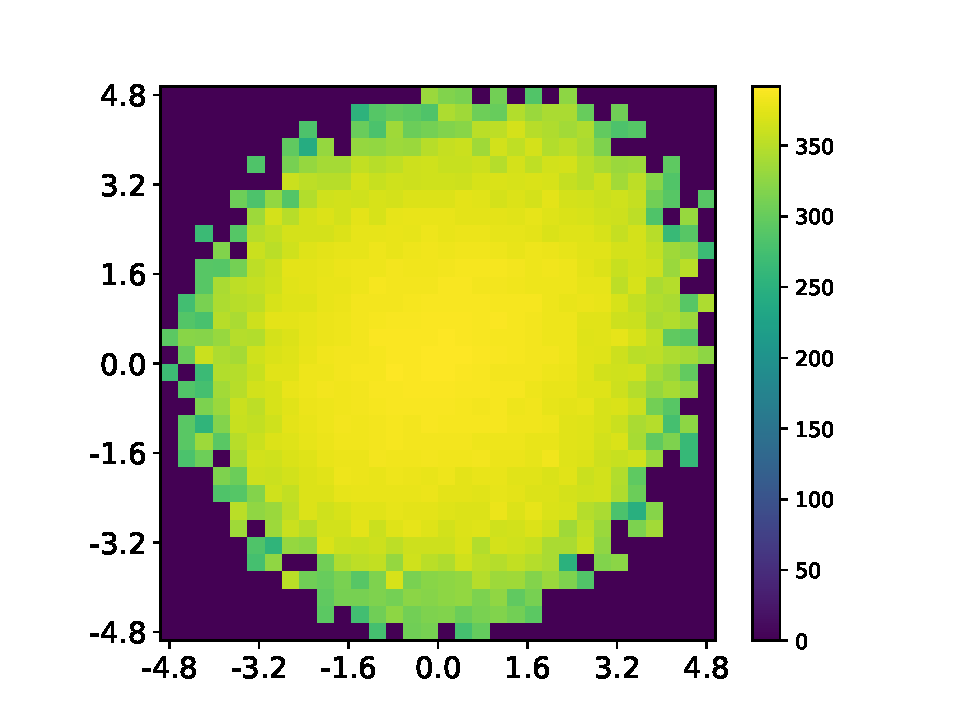
\includegraphics[width=0.45\textwidth]{original_map_elites.pdf}
\caption{The resultant repertoire after 4000 MAP-Elites iterations.
The coordinates correspond to the 2D displacement brought by each policy, and the color indicates the fitness score.
Policies leading to smaller displacements have bigger fitnesses as they require lesser electric cost.
}
\label{original_repertoire}
\end{figure}









\subsection{Determine the Coordinates of Policies}
After having generated the repertoire, we can evaluate the policies in different simulation settings to get the distortion basis.
These basis will then follow a dimensional reduction via SVD and finally converted into the coordinate system using PCA transform.
To prepare a wide range of environments to collect distortions, we selected 6 environments for each damage condition (intact case and four damaged cases for four legs), where the friction and torque ratio (to model payload) for each environment are randomly selected from a uniformly distribution between 0.7 to 1.
Thus, we acquired 30 different environments in total.
We then evaluate the entire repertoire in each one of the environments and record the dynamics representations for each policy.
There are two different representations of dynamics used in this paper, displacement-based and arc-based (see Fig \ref{baseline_trajectories}). 
The distortion is defined to be actual outcome minus the baseline, where our baselines are the dynamics representations recorded during the MAP-Elites evaluations.
The distortion for the direction $\varphi$ in arc-base representation is rather special due to the periodic nature of angles.
For example, if the baseline direction is $30^{\circ}$ and actual outcome is $330^{\circ}$, the distortion should be $-60^{\circ}$ instead of $300^{\circ}$.
Hence, we need to make sure that the directional distortion always lies between $-180^{\circ}$ to $180^{\circ}$.

\begin{figure}[h]
\centering
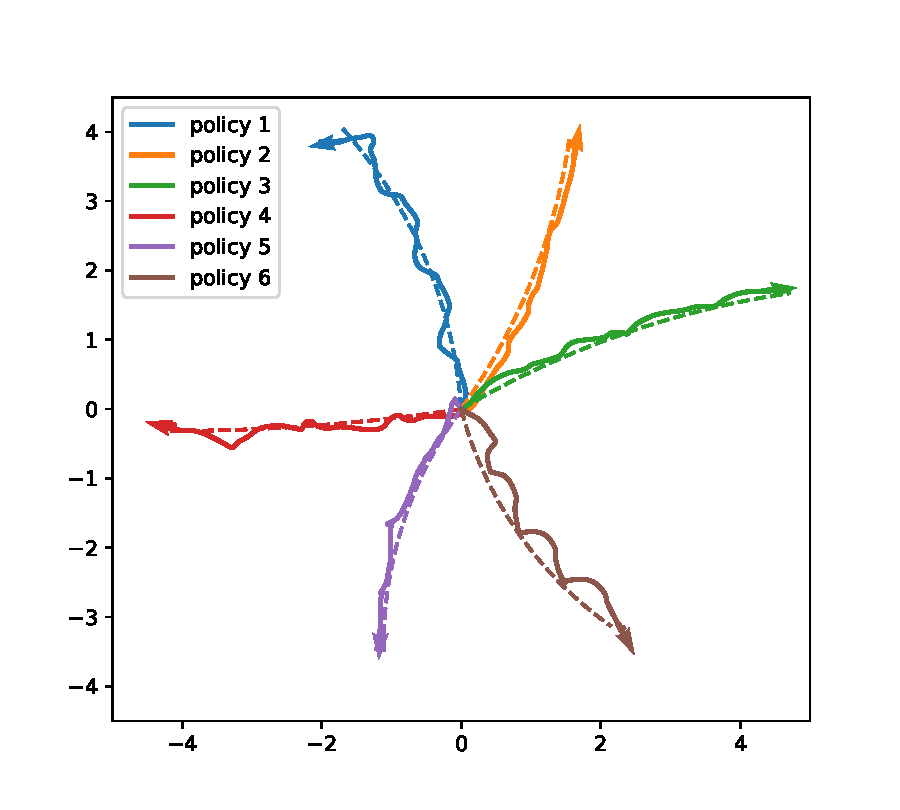
\includegraphics[width=0.45\textwidth]{original_trajectories_1.pdf}
\caption{The trajectories of 6 elementary policies in default simulation settings.
The dashed lines denote the predicted trajectories in arc-based representation with the parameters calculated using Eq. (\ref{all_three_parameters}).
The fact that the predicted curves stick closely to the actual trajectories indicates such representation being successful.
}
\label{baseline_trajectories}
\end{figure}


We then use the results to conduct dimensionality reduction via SVD.
For displacement-based representation, this is easy to achieve.
However, this is not applicable for arc-based representations since the measurement noises are different for different policies.
Hence, we take an alternative approach by finding the basis that minimizes the squared distance error.
This is inspired by the fact that regular dimensionality reduction via SVD is essentially minimizing the squared reconstruction error.
For displacement-based representation, minimizing the squared error for $x$ and $y$ displacements is equivalent to minimizing the squared distance error. 
To do this for arc-based representation, we know that the reconstructed distortion matrix can be expressed in the following form:
\begin{equation}
\begin{gathered}
%
\hat{\bm{A}} = \bm{A} \bm{U} \bm{P}
%
\end{gathered}
\label{SVD_for_arc}
\end{equation}
where $\bm{A}$ is the original distortion matrix of size $N \times n$, $\bm{U}$ is a $n \times s$ matrix, and $\bm{P}$ is a $s \times n$ matrix.
Matrix $\bm{A} \bm{U}$ gives the linear basis we are looking for, and matrix $\bm{P}$ reconstructs the original matrix from the basis.
This applies to all three parameters in arc-based representation, and we can calculate the predicted displacement from the reconstructed distortion matrix using Eq. (\ref{position_from_arc}).
Note that the matrix $\hat{\bm{A}}$ is the distortion, hence to recover the predicted parameters we need to add the baseline results.
To minimizes the squared error in distance, we used gradient descend to update the $\bm{U}$ and $\bm{P}$ matrix for each parameter.
This requires the initial values for the $\bm{U}$ and $\bm{P}$ matrix, which can be the ones found in SVD.
Hence, the initial $\bm{U}$ matrix is the same as in Eq. (\ref{ATA}), and the initial $\bm{P}$ matrix is $\bm{U}^T$.
We then ran the gradient descent for 2000 iterations with a learning rate of $0.0005$, and we finally took the $\bm{A} \bm{U}$ matrix as our basis.


To determine the number of dimensions we need, we plotted out the error against the dimension number in Fig \ref{original_elbow}.
We then used elbow method \cite{elbow} to determine the dimension number to be 5.
However, we can see from this plot that the remaining error is still quite large especially for arc-based representation.
A deeper investigation tells that this is because some policies are very noisy, and their outcomes seem to be not predictable.
Hence, we filter out the policies with squared errors larger than 3.
This leaves us with 398 remaining policies, and we replotted the curve in Fig \ref{filtered_elbow}.
We can see that the elbow is still at 5 while the error is greatly reduced.
The two curves also become closer, although the remaining error for arc-based representation is still larger.
To check that our filtering does not harm the coverage of the repertoire, we plotted out the remaining polices in task space (see Fig \ref{filtered_repertoire}).
We can see that our filtering does create some vacancies, but overall the task space is still well covered.
Finally, we use PCA transform to convert the basis into the coordinates in the input space.


\begin{figure}[h]
\centering
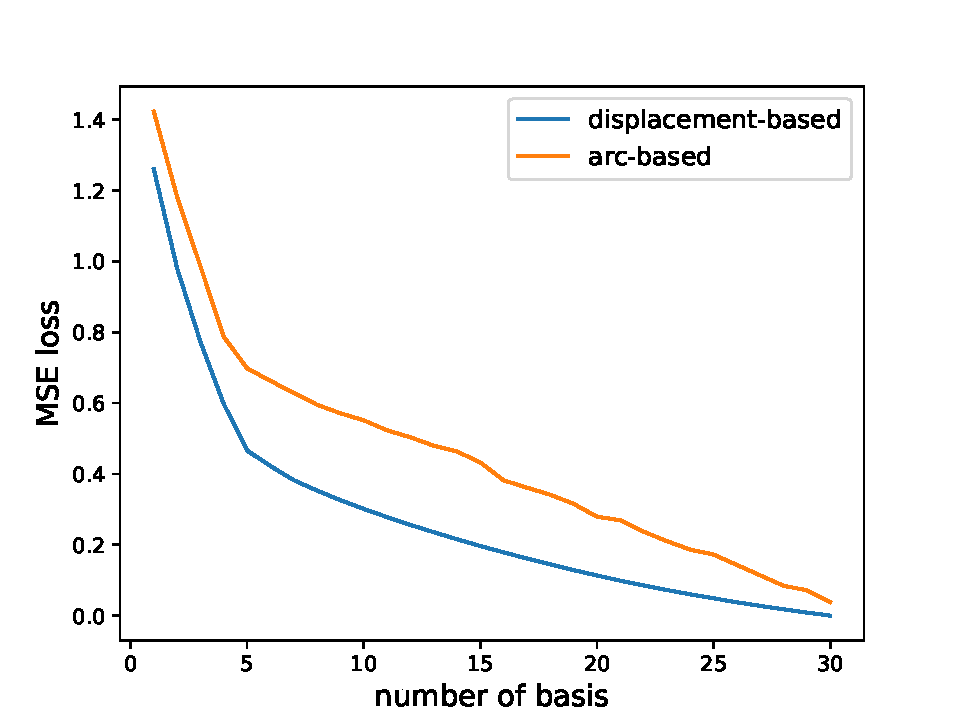
\includegraphics[width=0.45\textwidth]{elbow.pdf}
\caption{The mean squared distance error against the number of basis.
The elbows for the two curves are both at 5.  
}
\label{original_elbow}
\end{figure}


\begin{figure}[h]
\centering
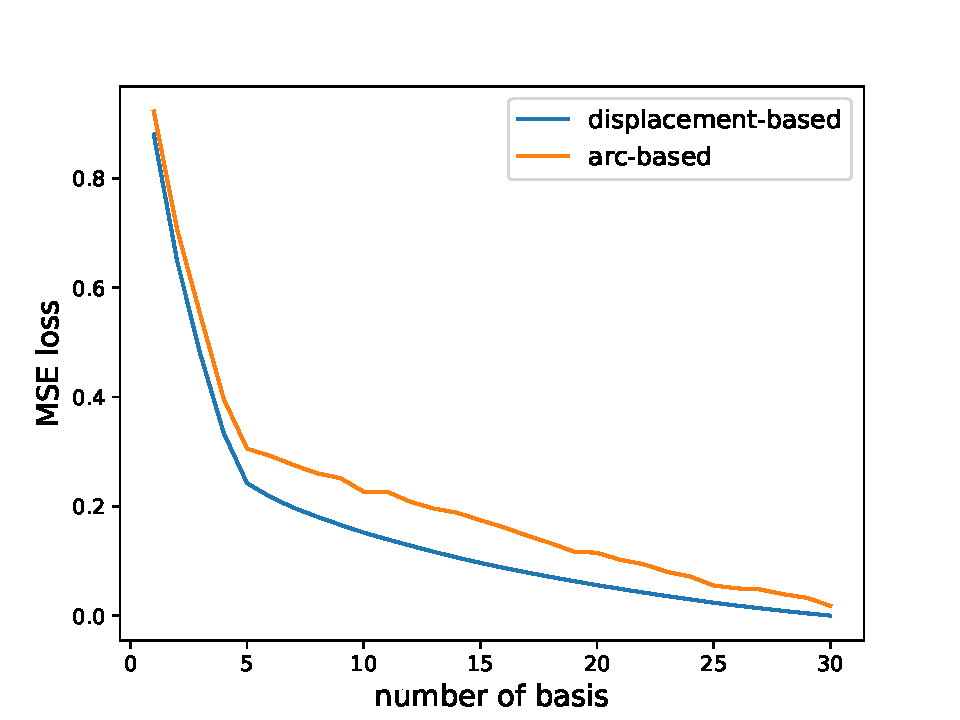
\includegraphics[width=0.45\textwidth]{filtered_elbow.pdf}
\caption{The mean squared distance error against the number of basis after filtering out the policies with large errors.
}
\label{filtered_elbow}
\end{figure}

\begin{figure}[h]
\centering
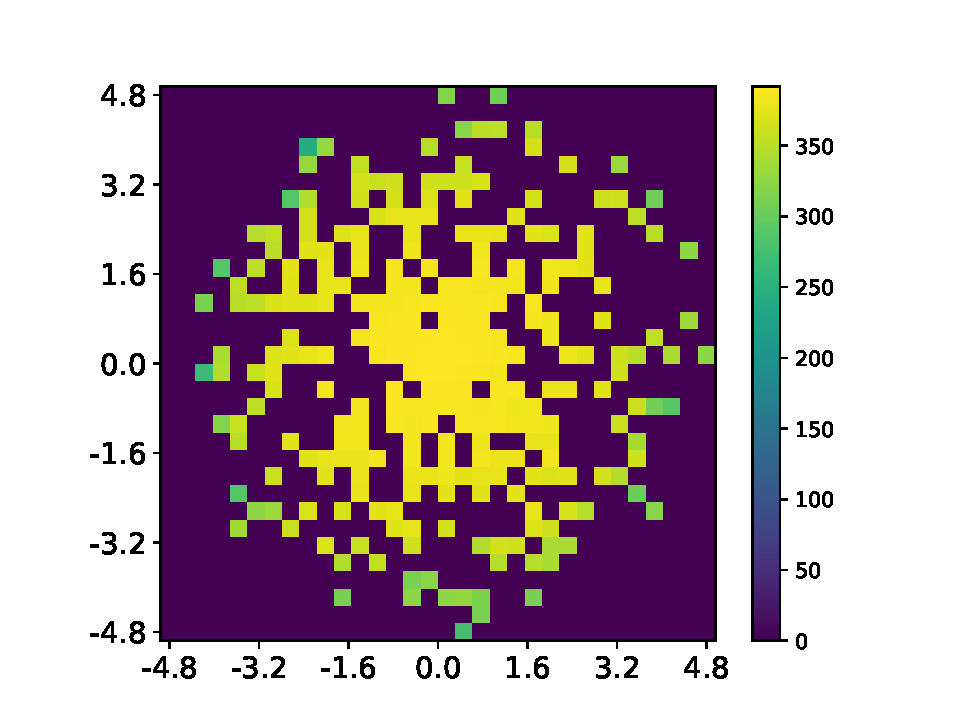
\includegraphics[width=0.45\textwidth]{filtered_map_elites.pdf}
\caption{The remaining repertoire after filtering.
}
\label{filtered_repertoire}
\end{figure}







\subsection{Clustering the Collaboratively Collected Data}
We can then evaluate our collaborative learning algorithm by clustering some collaboratively collected data and testing the adaptation performance. 
First, we need to conduct the Monte Carlo sampling required by DP clustering.
To do this, we randomly sampled 128 environments with 64 interaction data for each environment.
The damage status of these environments is evenly distributed for five damage conditions, and the friction and the torque are both uniformly distributed from 0.7 to 1.
The model parameters for each sample are determined with MLE.
One thing to notice is that, although our kernel should be Matern $\frac{5}{2}$ since we have assumed the dynamics to twice differentiable when deriving the linear prior mean function, it is found that Matern $\frac{3}{2}$ fits better to our data.
This is likely because the noises are also incorporated in the basis of our prior mean function, which harms the smoothness of the residual.
After having determined the priors of model parameters, we can test our clustering method on real-world data.
However, the collection of real-world data is too expensive for this project, hence we simulated this by randomly sampling a few episodes of data from several simulated environments.
The details about these environments can be found in Table \ref{data}.
Since we do not require the data to come from the same environment, we add a small noise to the environment parameters each time we sample an episode.
Considering the fact that the length of the episodes are not necessarily consistent, the length of each episode randomly fluctuates from 6 to 20.
We then performed 200 Gibbs sweeps to identify the configuration of cluster assignment with the largest posterior likelihood.
During clustering, the concentration parameter $\alpha$ is 1, and the threshold of the data size to apply posterior convergence is set to 30.

\begin{table}
\caption{Collaboratively Collected Data}
\centering
\def\arraystretch{1.2}
\begin{tabular}{|c||c|c|c|c|}
\hline
Label & env 1 & env 2 & env 3 & env 4\\
\hline
Damage & intact & leg 1 & leg 2 & leg 3 \\
\hline
Friction & 0.95 $\pm$ 0.01 & 0.85 $\pm$ 0.01 & 0.73 $\pm$ 0.01 & 0.88 $\pm$ 0.01 \\
\hline
Torque & 0.95 $\pm$ 0.01 & 0.92 $\pm$ 0.01 & 0.90 $\pm$ 0.01 & 0.76 $\pm$ 0.01 \\
\hline
Amount & 20 & 10 & 5 & 15 \\
\hline
\end{tabular}
\label{data}
\end{table}



\subsection{Model-Based Adaptation in a Maze}
To test the adaptation performance, we deployed our robot in a maze (see Fig \ref{maze}) with unknown dynamics and let it navigate to the exit as fast as possible.
The robot knows its position and orientation at each time-step, but the outcomes of executing each policy need to be learned online.
The radius of the robot is 0.41.
If the distance to the closest obstacle is smaller than this value, the robot collides with the obstacle.
In this case, the robot will spend another time-step to return to its previous position.
Hence, having collision will waste two time-steps, but the robot can acquire the outcome of the policy that led to the collision.



To perform model-based adaptation, the robot uses a simple planning algorithm similar to the dynamic window approach \cite{DWA}.
In every time-step, the repertoire stands for all the possible actions that the robot can take.
The outcomes of those actions are predicted using the learned model.
These predicted outcomes are then evaluated by an objective function:
\begin{equation}
\begin{gathered}
G(\bm{s}, \hat{\bm{s}}') = \operatorname{heading}(\hat{\bm{s}}') - 
\operatorname{penalty}(\operatorname{dist}(\hat{\bm{s}}')) \\
- k \cdot \operatorname{collision}(\bm{s}, \hat{\bm{s}}')
\end{gathered}
\label{objective_function}
\end{equation}
where $\bm{s}$ denotes the current state of the robot, and $\hat{\bm{s}}'$ stands for the predicted subsequent state by executing the elementary policy.
The term $\operatorname{heading}(\hat{\bm{s}}')$ quantifies the alignment of the action with the target, and the $\operatorname{penalty}(\operatorname{dist}(\hat{\bm{s}}'))$ term penalizes the distance to the closest obstacle.
The last term $\operatorname{collision}(\bm{s}, \hat{\bm{s}}')$ is a binary function that returns $1$ if transition $\bm{s} \rightarrow \hat{\bm{s}}'$ leads to collision and $0$ otherwise.
$k$ is a large positive value to give a large penalty for collision.
The robot uses this objective function to evaluate all the elementary policies and executes the one with the highest result.
After execution, the robot updates its state $\bm{s}$ as well as the dynamics model before taking the next step.
This process is repeated until the robot reaches the exit or runs out of time.



In our implementation, the state $\bm{s}$ refers to the position of the robot. 
The dynamics model predicts the 2D displacement for each policy, which is then converted into the subsequent state $\hat{\bm{s}}'$ using the following formula:
\begin{equation}
\hat{\bm{s}}' = \bm{s} + 
\begin{bmatrix}
\cos (\theta) & -\sin(\theta) \\
\sin (\theta) & \cos(\theta) \\
\end{bmatrix}
%
\begin{bmatrix}
\Delta \hat{x} \\
\Delta \hat{y} \\
\end{bmatrix}
\label{predicted_subsequent_state}
\end{equation}
where the $\theta$ is the orientation of the robot.
For arc-based dynamics representation, the predictions need to be transformed into displacement using Eq. (\ref{position_from_arc}).
There is a problem that the predicted outcome given by Eq. (\ref{simplified_distortion}) is not a value but a mixture of Gaussian distributions.
For simplicity, we just used the mean as the predicted result, which is a linear combination of the means for each Gaussian:
\begin{equation}
\begin{gathered}
\hat{x}^*_d 
= \sum_j p(c=j| \bm{x}_{1:N}) \mu(x^*_d|\bm{\theta}^*_j, \bm{x}_{1:N})
\\
+ \,\, p(c \neq j, \forall j|\bm{x}_{1:N})  \mu(x^*_d|\bm{x}_{1:N}, \text{RTE})
\end{gathered}
\label{predicted_mean}
\end{equation}
In practice, it is found that the RBF kernel used in the original RTE method \cite{RTE} severely overestimates the smoothness.
As a result, we used Matern $\frac{1}{2}$ with prior variance set to $4$ instead.
The $\operatorname{heading}(\hat{\bm{s}}')$ term in the objective function is defined to be the effective travelled distance, which is the projection on the suggested path.
The distance penalty is a specially designed function:
\begin{equation}
\begin{gathered}
\operatorname{penalty}(x) = \frac{0.162}{(x - 0.23)^2}
\end{gathered}
\label{penalty}
\end{equation}
Such design is to satisfy two important properties.
First, $\frac{d}{d x} (\operatorname{penalty})|_{(0.41 + 0.5)} \approx -1$.
Since $|\nabla(\operatorname{heading})| \leq 1$, this suggests that the sum of the first two terms in $G(\bm{s}, \hat{\bm{s}}')$ is sure to decrease when the distance is smaller than $0.5 + 0.41$.
Hence, we have inexplicitly defined the safe distance to be 0.5 to account for the uncertainties in model predictions.
The second property is that $\operatorname{penalty}(0.41) = 5$. 
This means that when the robot is about to collide, the penality will exceed the maximum increase in $\operatorname{heading}$ that can happen in one time-step, which is 4.8.
Finally, coefficient $k$ in the last term is set to 100.




 



\begin{figure}[h]
\centering
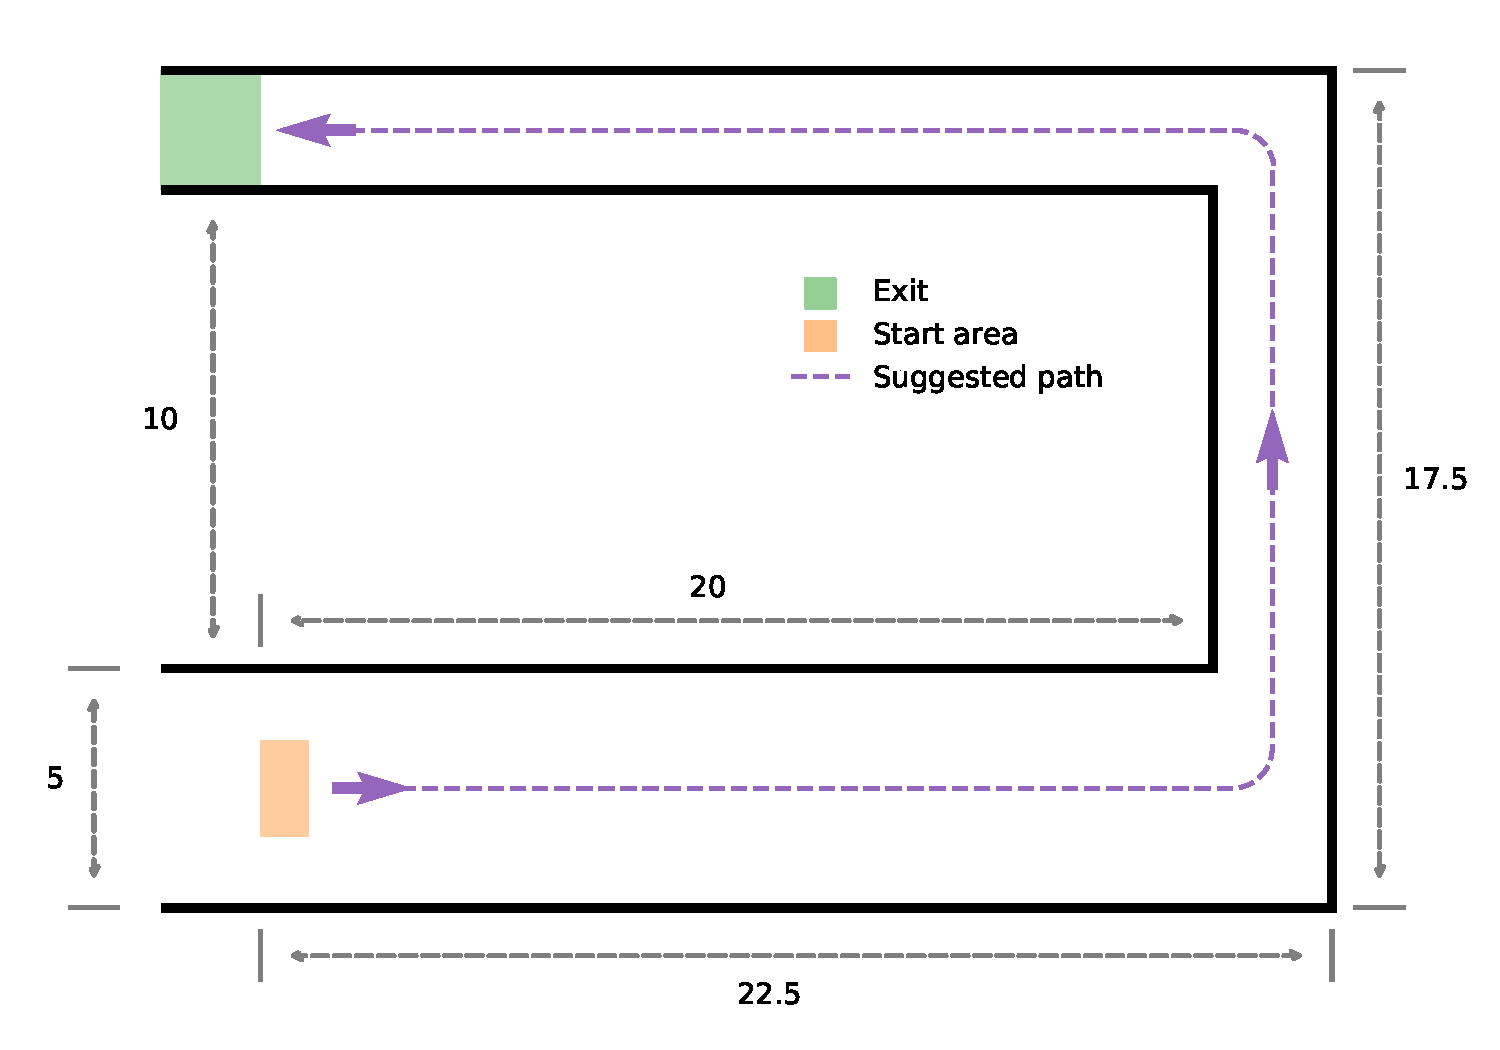
\includegraphics[width=0.45\textwidth]{tunnel_floorplan.pdf}
\caption{The floor-plan of the maze.
The starting area is a rectangle with width equals to 1 and height equals to 2.
To allow some exploration at start, the width of the tunnel is 5 before the first turning and then reduces to 2.5 for the rest of the sections.
}
\label{maze}
\end{figure}
















\section{Results and Analysis}

\subsection{Dirichlet Process Clustering}
The result of our clustering is presented in Fig \ref{clustering_results}.
We can see that the method managed to accurately group up the data from the same environment with only one miss classified episode in arc-based representation.
Further investigation shows this is a rather small episode containing only 9 interaction data. 
It is likely that when expressed in arc-based representation, the data in this episode happen to exhibit similar outcomes in both environments which finally led to this confusion.
However, another feature of the clustering result is that data from the same environment can spread in multiple clusters, and we even have many clusters containing only one episode.
There are two possible reasons for this phenomenon.
One is that some execution is very noisy, hence if an episode happens to include such interaction data, it might appear to be largely different from the rest of the episodes.
Another possible reason is that we applied posterior convergence too soon, and the weights calculated using Eq. (\ref{refitted_weights}) over-fits to the existing data, hence preventing further data from joining the cluster.
Fortunately, this should not affect the model prediction too much.


\begin{figure}[h]
\centering
\subfloat[]{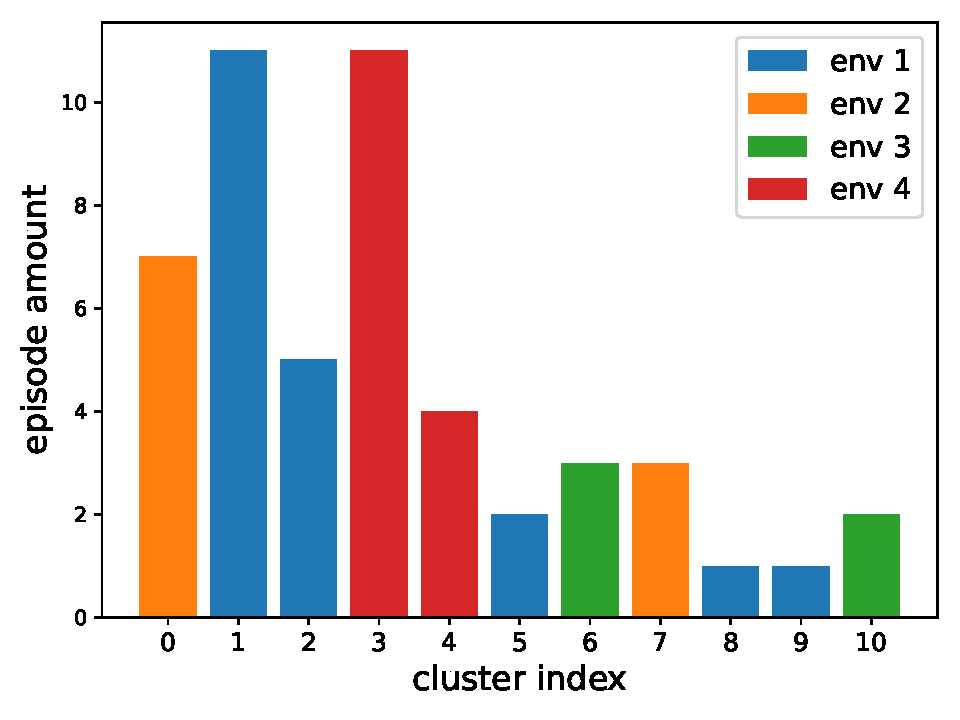
\includegraphics[width=0.22\textwidth]{xy_cluster_data.pdf}
%\label{a}
}
%\hfil
\subfloat[]{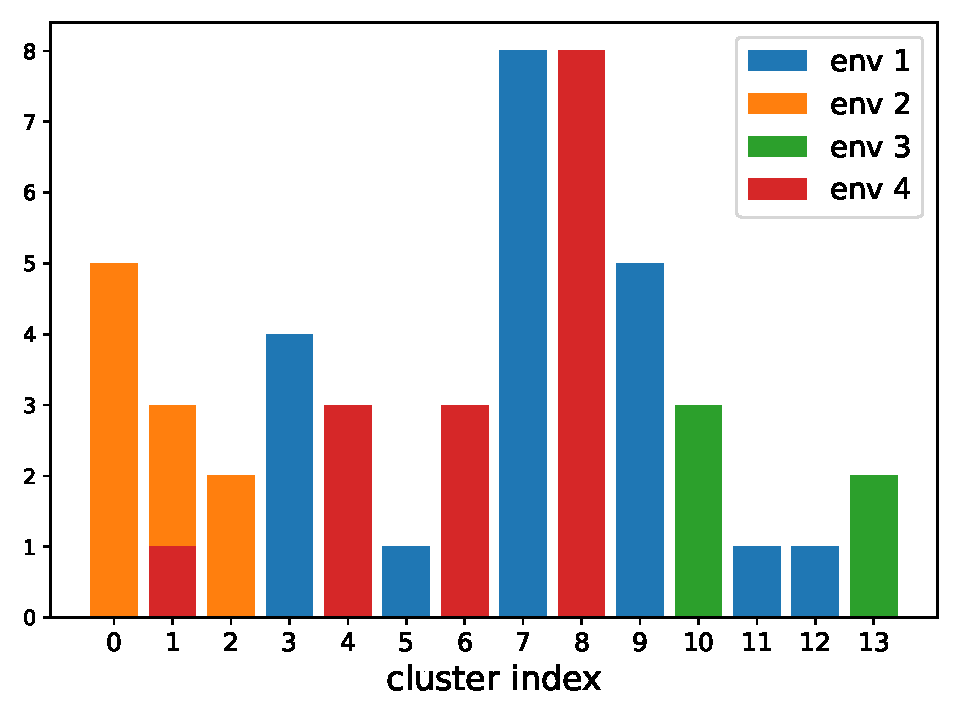
\includegraphics[width=0.22\textwidth]{arc_cluster_data.pdf}
%\label{b}
}
\caption{Cluster assignment of the data in Table \ref{data} after applying our DP clustering method.
(a) is the result using displacement-based representation, and (b) is the one for arc-based representation.}
\label{clustering_results}
\end{figure}


\begin{figure*}[!t]
\centering
\subfloat[]{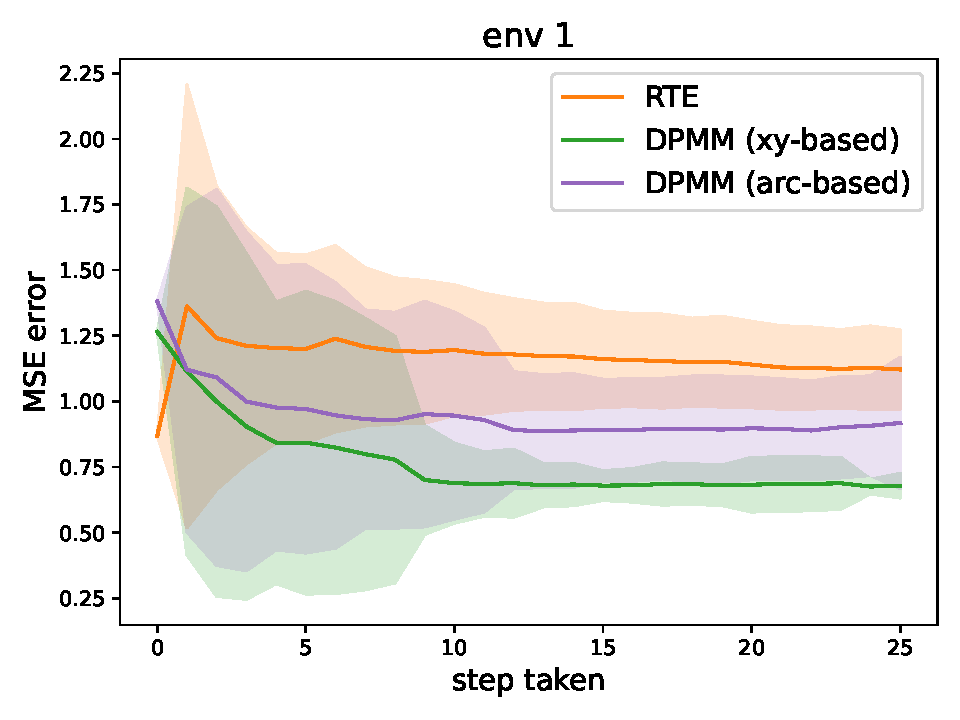
\includegraphics[width=0.45\textwidth]{regular_case0.pdf}%
\label{case_0}}
%\hfil
\subfloat[]{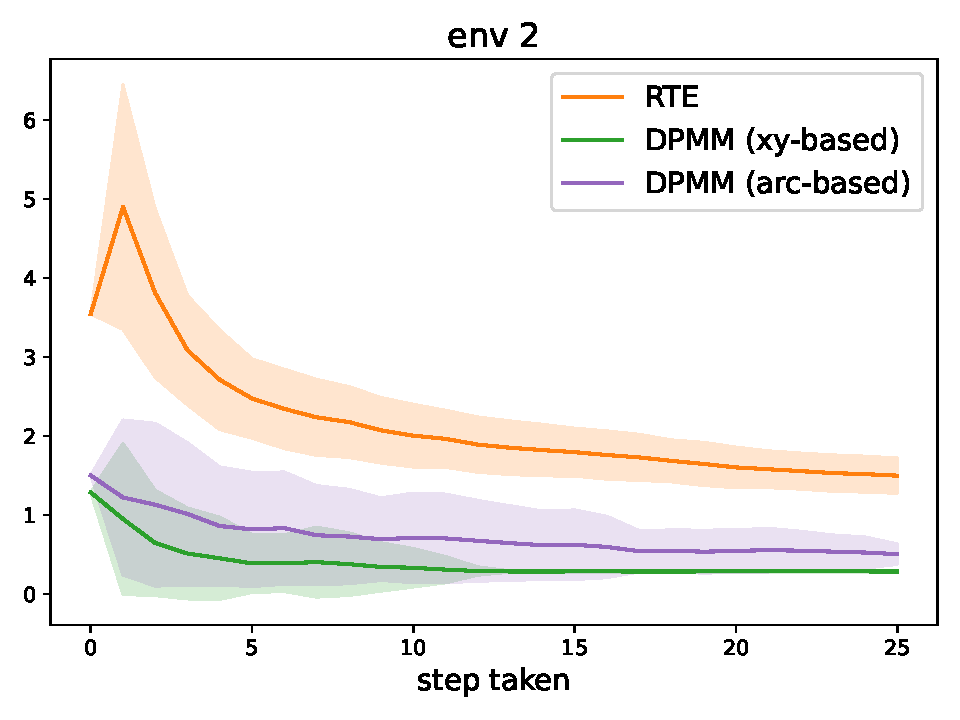
\includegraphics[width=0.45\textwidth]{regular_case1.pdf}%
\label{case_1}}
\vfil
\subfloat[]{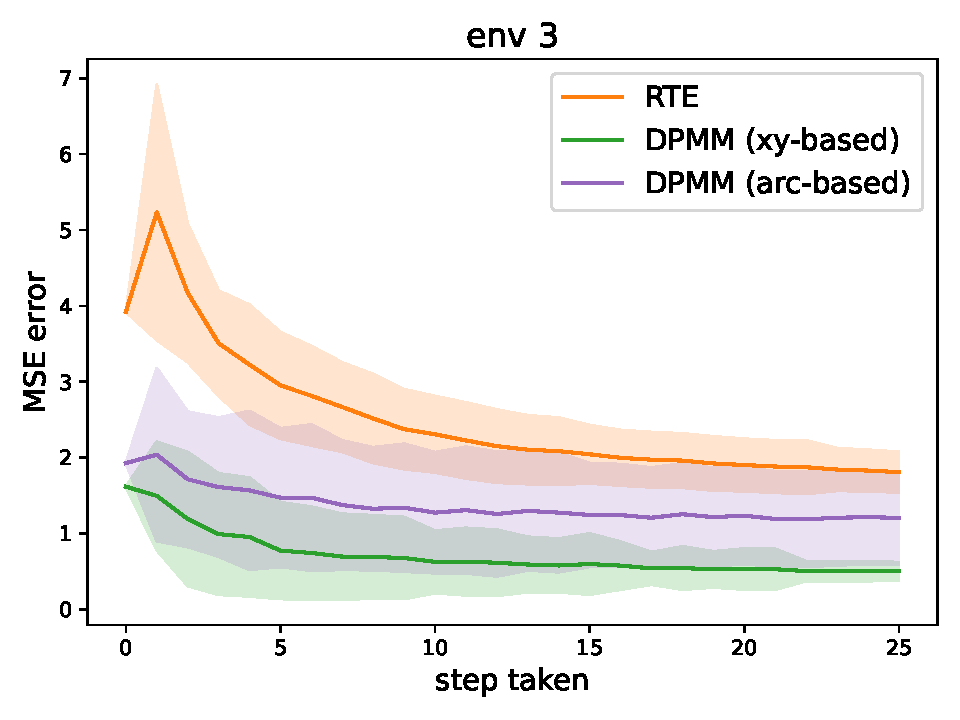
\includegraphics[width=0.45\textwidth]{regular_case2.pdf}%
\label{case_2}}
%\hfil
\subfloat[]{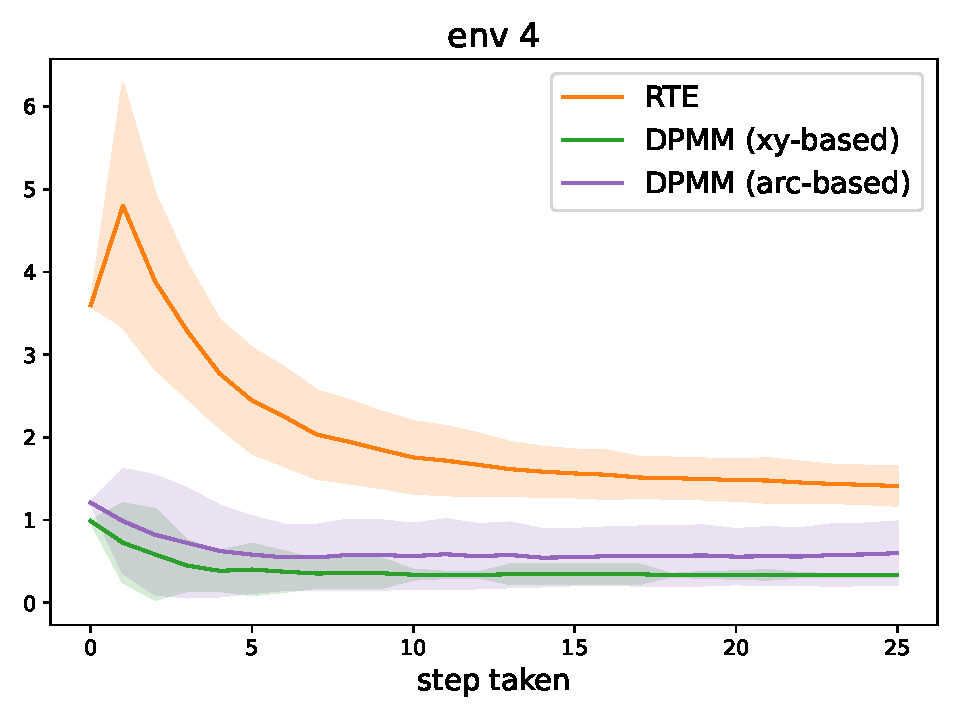
\includegraphics[width=0.45\textwidth]{regular_case3.pdf}%
\label{case_3}}
\caption{The prediction error versus the step taken in each environment.
The error is defined to be the mean-squared distance between the predicted final position and the actual final position.
}
\label{dynamics_learning}
\end{figure*}

\subsection{Dynamics Learning}
Before deploying the robot in the maze, we first test the capability of our robot to quickly learn the dynamics using the infinite mixture of GP model.
We do this by placing our robot in a previously encountered environment and feeding the robot with a randomly selected interaction data in each step.
We then make the robot predict the outcomes for the entire repertoire and monitor the change of the prediction error.
This is to simulate the model-based online adaptation process where the robot executes a policy in each time-step and use the outcome to update its model.
To mitigate the randomness in the result, we repeat this 100 times and plotted out the mean and standard deviation in Fig \ref{dynamics_learning}.


We can see that for any previously encountered environment, our model greatly outperforms the RTE method.
Surprisingly, the displacement-based method is significantly better than the arc-based method.
The displacement-based method can typically reduce the error to below $1.0$ within 5 steps, while the arc-based method learns much slower and is lesser stable.
This could result from the fact that arc-based method uses three parameters unlike the use of two parameters in displacement-based representation.
It's likely that the extra dimension and the inconsistent measurement error in arc-based method induces more uncertainties than displacement-based approach and also make the selection of the prior lesser stable.
Nevertheless, both infinite mixture of GP methods are much better than RTE.
This suggests that it is a successful method to identify candidate priors from the historical data and try to figure out the most suitable prior with the data collected online.
We also see that the RTE starts up with a increase in error.
This is likely a sign that the use of $x$ and $y$ displacements as the input space fails to handle the case where two policies leading to similar displacements in the default simulation environment create distinct outcomes in a new environment.
This explains the rapid increase in the error as such input space could generate misleading result.
It is counter-intuitive to see that env 1 has the largest error while it is most similar to the default environment.
Further investigation finds it hard to achieve an error lesser than 0.6 in env 1.
It is also found that environments closer to the default one have larger uncertainties in policy execution.
This is likely because the effect of random perturbation will accumulate during the motion, and the faster the robot walks the greater the uncertainties will be.
The data size collected from each environment matters as the learning in env 4 (15 episodes) is the fastest, while that in env 3 (5 episodes) is slowest.

\begin{figure*}[!t]
\centering
\subfloat[]{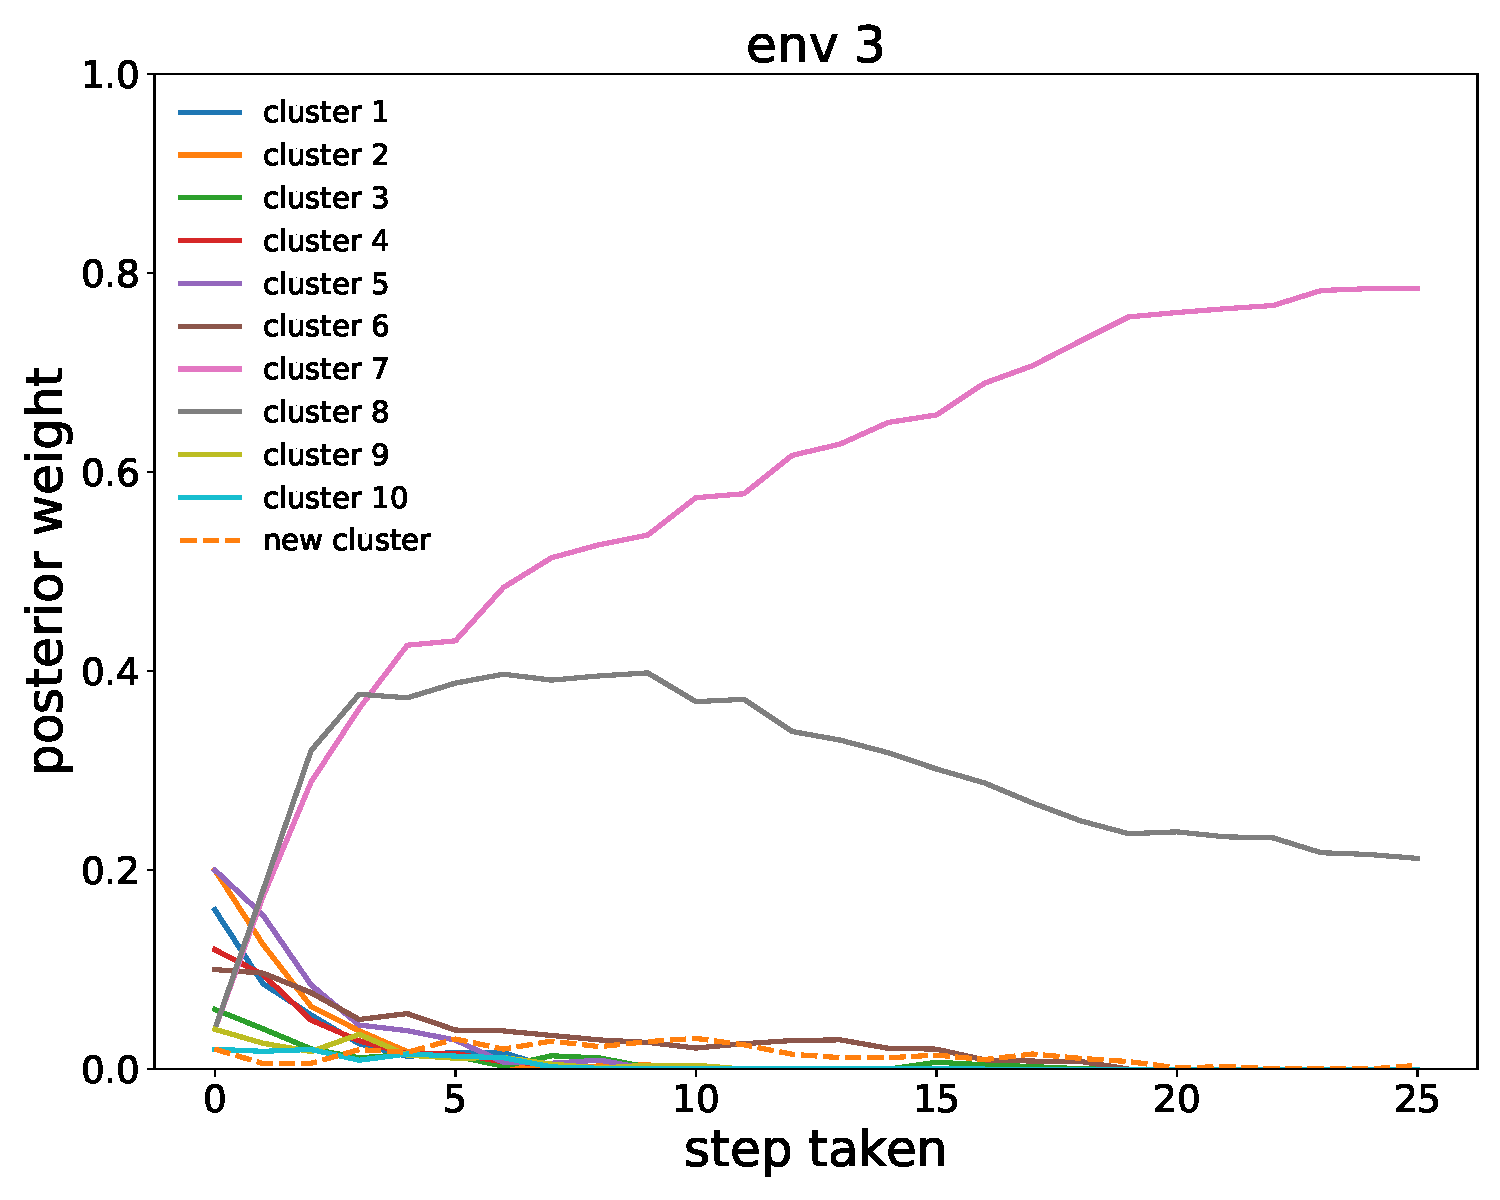
\includegraphics[width=0.45\textwidth]{weight_2.pdf}%
\label{weight_2}}
%\hfil
\subfloat[]{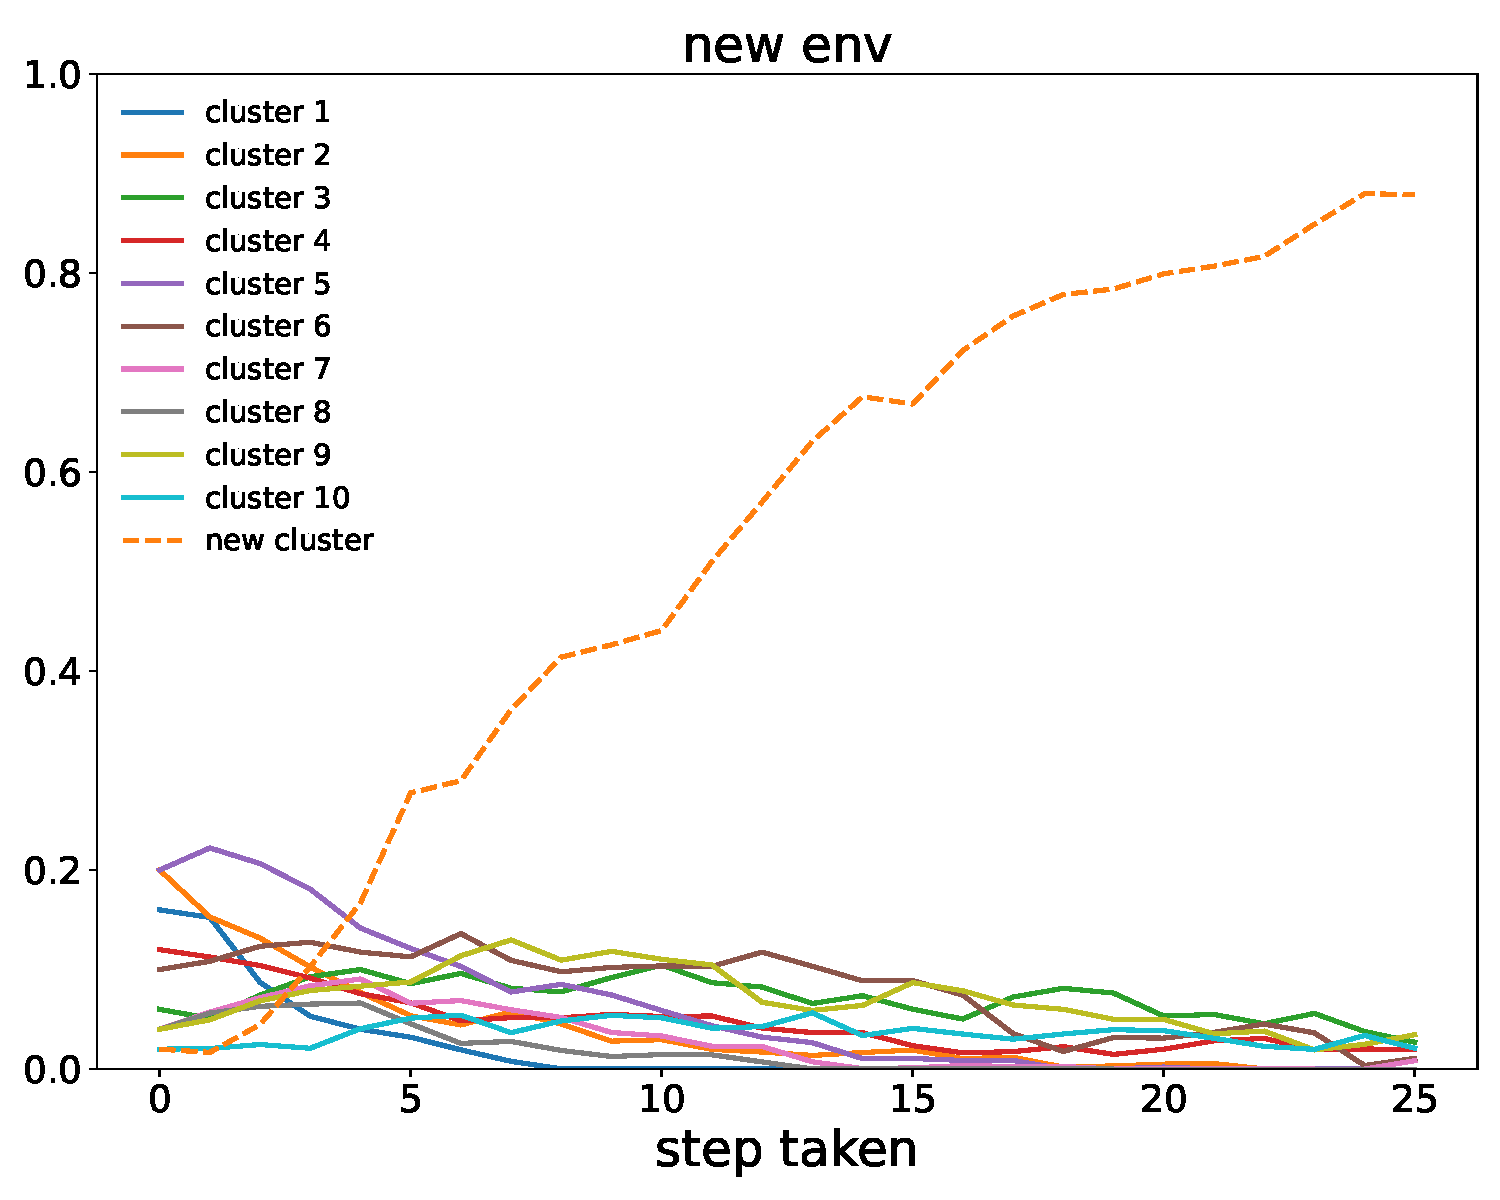
\includegraphics[width=0.45\textwidth]{weight_4.pdf}%
\label{weight_4}}
\caption{The change of the posterior weight of each cluster versus the number of steps taken.
These data correspond to the model using displacement-based dynamics representation.
}
\label{weights}
\end{figure*}

\begin{figure}[h]
\centering
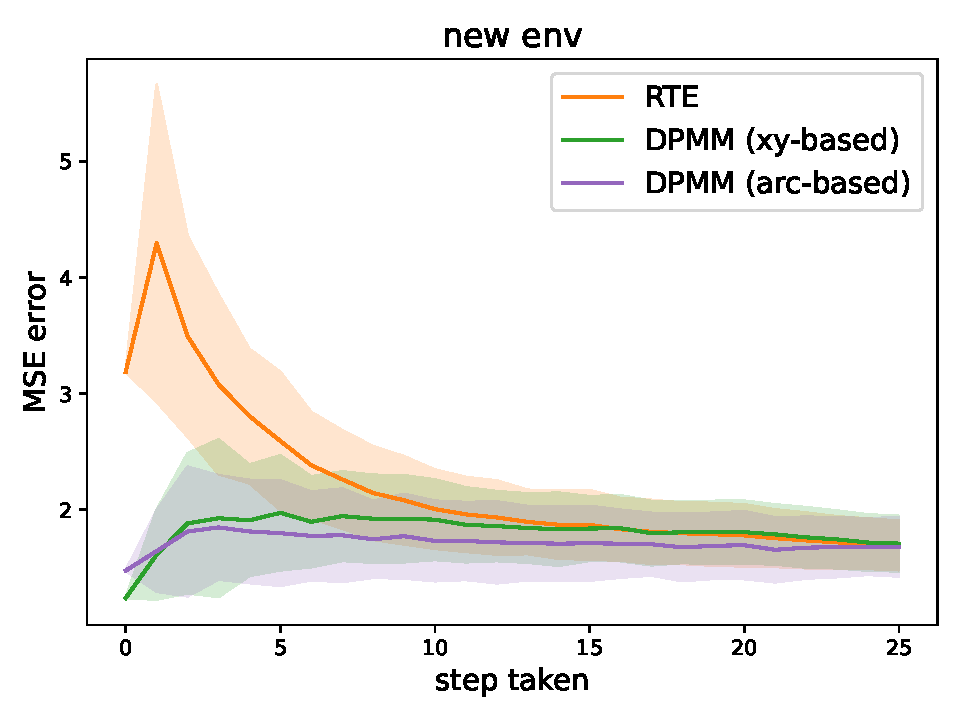
\includegraphics[width=0.45\textwidth]{regular_case4.pdf}
\caption{Dynamics learning in an unseen environment.
For this environment, the robot damage is in the leg 4, the friction coefficient is 0.77 and the torque scale is 0.82}
\label{new_env}
\end{figure}

These online learnings are all made in previously encounter environments.
To examine the generalizability of our method, we also tested the adaptation on a new environment.
It can be seen from Fig \ref{new_env} that although this environment is new hence none of the historical data will help, our method still manges to adapt in this environment as good as RTE.
To monitor the selection of the prior during the adaptation, we plotted out the posterior weights of each cluster, namely the $p(c=j| \bm{x}_{1:N})$ in Eq. (\ref{predicted_mean}).
We see from Fig \ref{weight_2} that although the data for env 3 split into two clusters (see Fig \ref{clustering_results}), they collectively contribute to most of the posterior weights.
When deployed in the new environment, none of the existing clusters can explain the interaction data.
Thanks to the wonderful property of DP that the probability for getting a new cluster is never zero, we see from the posterior weights in Fig \ref{weight_4} that the robot eventually realizes that it is in a new situation and hence uses RTE to make prediction.


Finally, we tested our model's capability of learning new dynamics.
This is done by adding an episode of new data to our dataset and updating our model accordingly.
This episode is collected from the new environment in Fig \ref{new_env} and contains 35 data.
The result is presented in Fig \ref{new_adapt}.
We see that after incorporating this new episode into our dataset, the robot using displacement-based method quickly learns how to adapt in this new environment.
The arc-based method is also performing better, but it learns slower.

\begin{figure}[h]
\centering
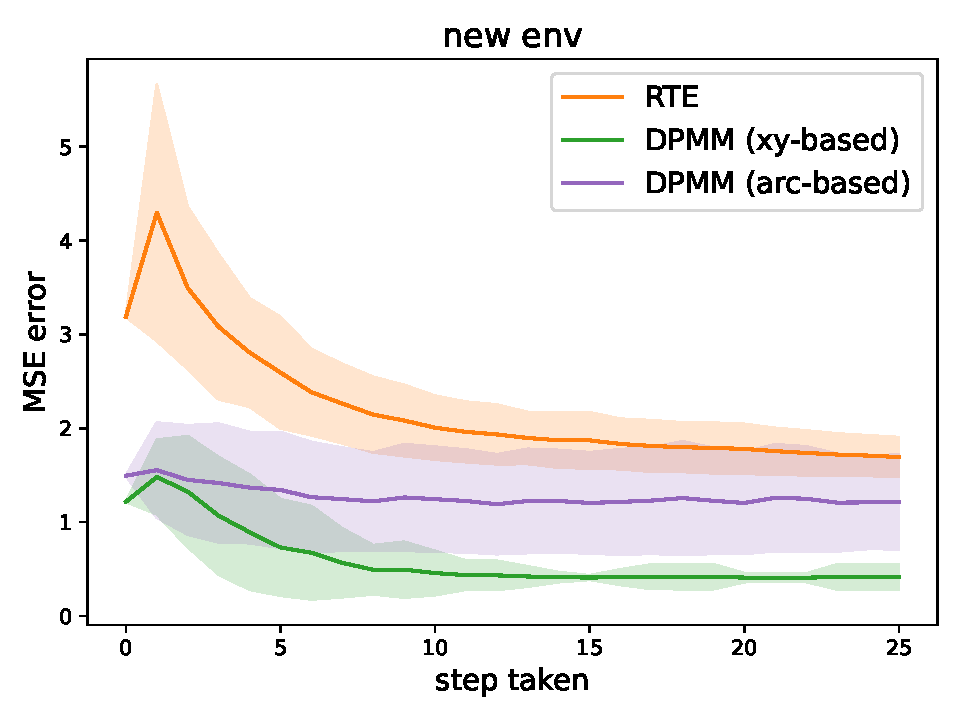
\includegraphics[width=0.45\textwidth]{new_case4.pdf}
\caption{Dynamics learning performance after having collected an episode of interactions from this environment.
With dataset updated, 20 extra Gibbs sampling sweeps were conducted to identify the best indicator configuration.}
\label{new_adapt}
\end{figure}


\begin{figure*}[!t]
\centering
\subfloat[]{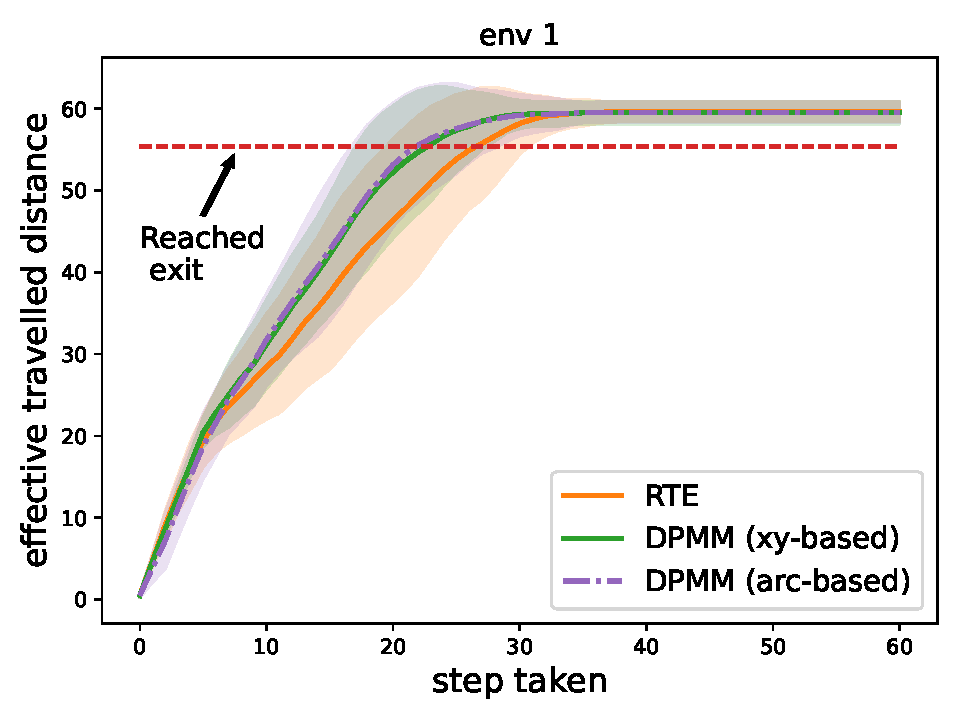
\includegraphics[width=0.45\textwidth]{navigation_results_0.pdf}%
\label{maze_0}}
%\hfil
\subfloat[]{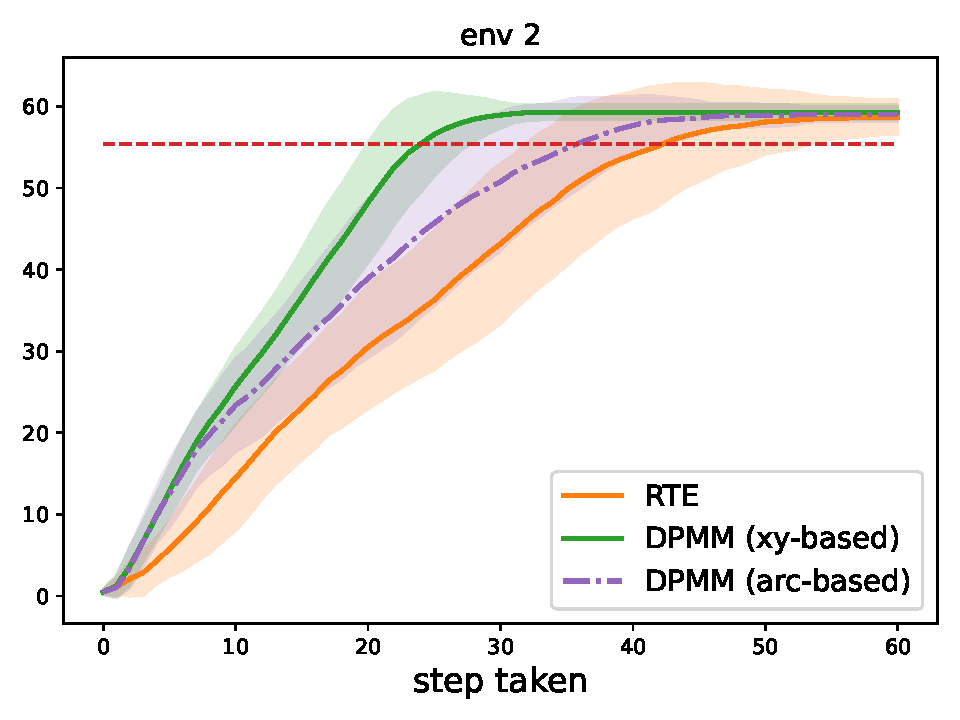
\includegraphics[width=0.45\textwidth]{navigation_results_1.pdf}%
\label{maze_1}}
\vfil
\subfloat[]{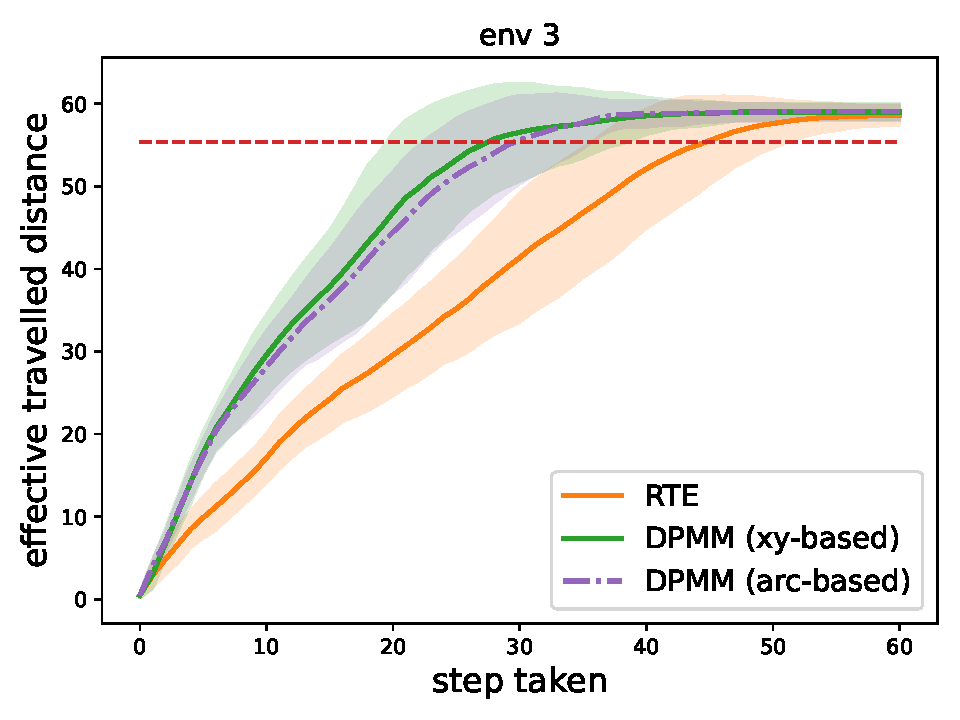
\includegraphics[width=0.45\textwidth]{navigation_results_2.pdf}%
\label{maze_2}}
%\hfil
\subfloat[]{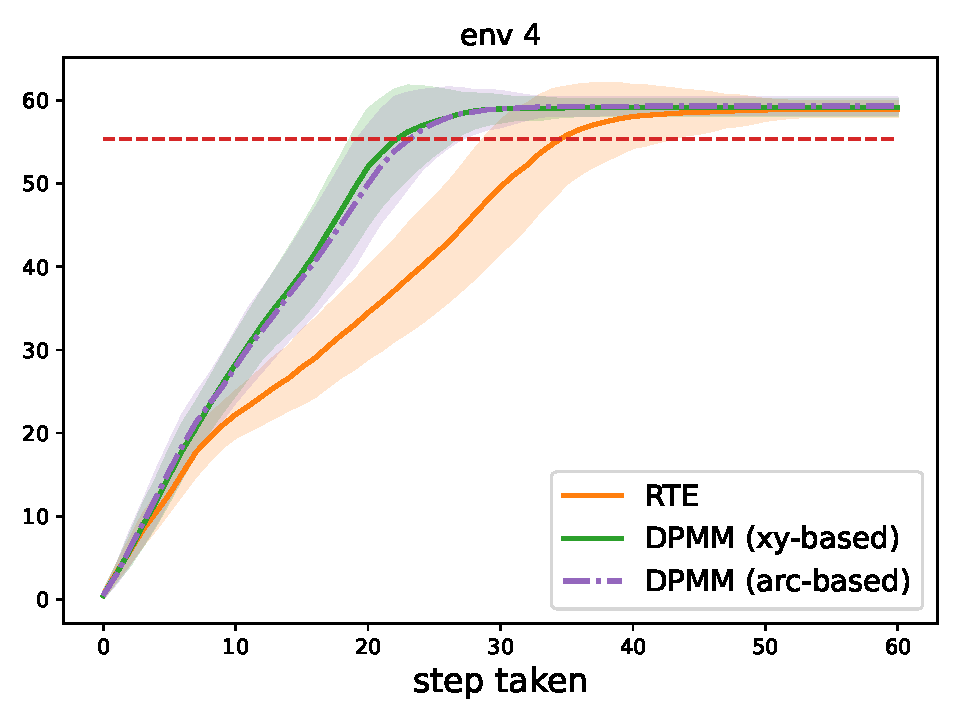
\includegraphics[width=0.45\textwidth]{navigation_results_3.pdf}%
\label{maze_3}}
\caption{The effective distance travelled by the robot versus the step number.
Since the maze is U-shaped, we use effective distance instead of the distance to the goal to track the progress of the robot.
The effective distance is defined to be the projection on the suggested path, which is the distance on the path that is closet to the robot's current position.
The effective distance at the exit is 55.386.
}
\label{navigation_results}
\end{figure*}


\subsection{Maze Adaptation}


Since our method shows very promising result in dynamics learning, we hoped to
investigate the practical significance of this improvement in actual task solving.
We deployed our robot in each of the previously encountered environments and let it navigate through the maze.
The results are presented in Fig \ref{navigation_results}. 
We see that in all environments, the robots using our models completes the task significant faster than the one using RTE.
Although we have found that the displacement-based method provides much more accurate modelling of the dynamics than the arc-based method, the two robots showed little difference in performance except in env 2.
A very likely explanation for this is that for the policies that are used most often, the two methods provide similar accuracies.
By examining the plots, we see that most curves experience a decrease in its gradient at effective distance roughly equals to 20.
Referring to the floor-plan of the maze in Fig \ref{maze}, this effective distance corresponds to the first turning, after which the tunnel width is halved.
This poses a tougher requirement of the model predictions, which may otherwise lead to collisions.
We can see from Fig \ref{maze_0} and Fig \ref{maze_3} that the robot using RTE 
is not falling behind at start but fails to catch up after the first turning.
It is very likely that the model of the robot is not accurate enough for the narrowed tunnel and caused collisions during the motion.
We see from Fig \ref{maze_1} that the robot using arc-based method is likely suffering from similar issues in env 2.


To further analyse these results, the details of the maze adaptation are listed in Table \ref{detailed_data}.
We see that the robot using displacement-based method provides a very stunning improvement over RTE.
It takes around $35\%$ lesser steps to reach the goal except in env 1, where the dynamics is close to the baseline.
Similar improvement is offered by the arc-based method except for env 2.
By comparing the prediction error of the two methods, we see that for the policies that are executed during the adaptation, the two methods give very similar accuracies in their predictions except for env 2.
This is consistent with our speculation and explains the fact that the robot using arc-based method had $4.17$ more collisions in average when adapting in env 2.
However, it is strange that the arc-based method led to the most collisions in this environment, while RTE has much higher errors in its predictions.
A highly probably explanation for this is that while RTE provides much lesser accuracy, 


in many cases it chooses a policy that barely moves the robot but is also lesser likely to cause collisions.
 






\begin{table*}[t!]
\caption{Maze Adaptation Details}
\centering
%\def\arraystretch{1}
\begin{tabular}{c c c c c c c c c}
\hline
\addlinespace[0.1cm]
Method         & &       & DPMM xy-based & & DPMM arc-based & & RTE   & \\
\addlinespace[0.1cm]
\hline
\addlinespace[0.1cm]
               & & env 1 & $21.5 \pm 4.13$ & & $21.04 \pm 4.49$ & & $24.23 \pm 5.42$ & \\
Steps to reach & & env 2 & $23.52 \pm 3.36$ & & $32.21 \pm 8.01$ & & $37.61 \pm 8.75$ & \\
 the exit & & env 3 & $25.99 \pm 7.12$ & & $28.42 \pm 6.43$ & & $40.8 \pm 8.80$ & \\
               & & env 4 & $22.13 \pm 3.30$ & &  $22.93 \pm 3.78$ & & $33.38 \pm 4.86$   & \\
\addlinespace[0.1cm]
\hline
%
%
\addlinespace[0.1cm]
               & & env 1 & $3.64 \pm 1.99$ & & $3.35 \pm 2.07$ & & $5.06 \pm 2.49$ & \\
Number of      & & env 2 & $2.24 \pm 1.61$ & & $6.41 \pm 3.52$ & & $4.29 \pm 2.29$ & \\
collisions     & & env 3 & $2.72 \pm 2.01$ & & $4.6 \pm 2.46$ & & $3.73 \pm 2.81$ & \\
               & & env 4 & $1.31 \pm 1.49$ & & $2.07 \pm 1.76$ & & $2.91 \pm 1.91$   & \\
\addlinespace[0.1cm]
\hline
%
%
\addlinespace[0.1cm]
               & & env 1 & $57.459 \pm 1.70$ & & $57.262 \pm 1.85$ & & $57.447 \pm 1.91$ & \\
Total travelled& & env 2 & $57.669 \pm 2.05$ & & $58.077 \pm 2.60$ & & $59.833 \pm 3.08$ & \\
distance       & & env 3 & $57.754 \pm 2.02$ & & $57.546 \pm 1.88$ & & $60.921 \pm 2.46$ & \\
               & & env 4 & $56.822 \pm 1.60$ & & $ 57.683 \pm 1.59 $ & &  $58.4387 \pm 1.47$ & \\
\addlinespace[0.1cm]
\hline
%
%
\addlinespace[0.1cm]
               & & env 1 & $0.759 \pm 0.14$  & & $0.849 \pm 0.027$ & & $1.048 \pm 0.23$ & \\
Model prediction&& env 2 & $0.800 \pm 0.24$ & & $1.059 \pm 0.034$ & & $1.618 \pm 0.14$ & \\
error (RMSE)   & & env 3 & $1.122 \pm 0.27$  & & $1.162 \pm 0.024$ & & $1.479 \pm 0.22$ & \\
               & & env 4 & $0.709 \pm 0.17$ & & $0.678 \pm 0.021$ & & $1.346 \pm 0.14$ & \\
\addlinespace[0.1cm]
\hline
\end{tabular}
\label{detailed_data}
\end{table*}



\section{Conclusion}






%\begin{footnotesize}

\bibliographystyle{unsrt}
\bibliography{reference}
%\end{footnotesize}

%\end{multicols}
\end{document}